\documentclass[12pt]{article}

\usepackage[a4paper,scale=0.8]{geometry}
\usepackage[english]{babel} % needed for English texts
\usepackage[utf8]{inputenc} % unicode encoding
\usepackage{amsmath,amssymb,amsfonts,amsthm}
\usepackage{stmaryrd}
\usepackage{listings}
\usepackage{bussproofs}
\usepackage{hyperref}  % automagically makes clickable references, table of contents
\usepackage{thmtools}
%\usepackage{enumerate} % enumerate replaced by enumitem
\usepackage[shortlabels]{enumitem}
%\usepackage[a4,frame,center,noinfo]{crop}	% frame around pages
\usepackage{setspace}
\usepackage{pdfpages}


\newtheorem{definition}{Definition}[section] % defines the definition environment
\newtheorem{theorem}{Theorem}[section] % defines the theorem environment
\newtheorem{lemma}{Lemma}[section]
%\newtheorem{proof}{Proof}[section] % defines the proof environment

% Sets and set operation
\newcommand{\R}{\mathbb{R}} % the reals
\newcommand{\Z}{\mathbb{Z}} % the integers
\newcommand{\N}{\mathbb{N}} % the natural numbers
\renewcommand{\S}{\mathbb{S}} % state space
\newcommand{\leqD}{\sqsubseteq_{D}} % cpo
\newcommand{\leqL}{\sqsubseteq_{L}} % cpo
%\newcommand{\pot}[1]{\mathcal{P}(#1)} % power set

\newcommand{\E}{\mathbb{E}}

% Programs
\newcommand{\smtx}[1]{\left\llbracket #1 \right\rrbracket} % semantic brackets
\newcommand{\res}[2]{\left\langle #1 \right\rangle_{#2}} % restriction
\newcommand{\resP}[1]{\res{#1}{B}} % restriction to B
\newcommand{\resN}[1]{\res{#1}{\lnot B}} % restriction to not B
\newcommand{\nop}{\textit{skip}} % skip statement
\newcommand{\abort}{\textit{abort}} % abort statement
\newcommand{\ifp}[3]{\textit{if}\,(#1) \, \{ \, #2 \, \} \, \textit{else} \, \{ \, #3 \, \} } % if statement
\newcommand{\while}[2]{\textit{while}\,(#1) \{#2\}} % while loop

\newcommand{\wh}{\operatorname{wh}_{B, P}}
\newcommand{\hh}{\operatorname{H}_{B, P}}
\newcommand{\ww}{\operatorname{ww}_f}
\renewcommand{\wp}[1]{\operatorname{wp}\l( #1 \r)}

% Convenience
\newcommand{\qu}{\frac{1}{4}} % 1 / 4
\newcommand{\half}{\l( \frac{1}{2} \r)} % (1 / 2)
\newcommand{\hf}{\frac{1}{2}} % 1 / 2
\newcommand{\IH}[1]{\overset{IH}{#1}} % for induction hypothesis
\newcommand{\pair}[1]{\left( #1 \right)} % round parentheses
\renewcommand{\l}{\left} % short left
\renewcommand{\r}{\right} % short right
\newcommand{\infsum}{\sum\limits_{i = 0}^{\infty}} % sum from 0 to inf over variable i
\newcommand{\multisum}[1]{\sum\limits_{s \in \N^k} #1 X_1^{s_1} \cdots X_k^{s_k}}
\newcommand{\Xok}{X_1^{s_1} \cdots X_k^{s_k}} % variables X_1 to X_k
\newcommand{\explain}[1]{\hspace*{2em} \l(\text{\small #1}\r)} % explanation in proof, indented line with smaller text
\newcommand{\where}{, \text{ where }}

% Display
\renewcommand{\vert}{\ | \ }

% Bussproofs spacing around horizontal line
\renewcommand{\extraVskip}{5pt}

\addtolength{\jot}{0.5em} % increase align line spacing

\newcommand{\HRule}{\rule{\linewidth}{0.5mm}}	% horizontal lines for title

% math symbol for general cartesian product, copied from kpfonts.sty, lines 611 & 1495
\DeclareSymbolFont{largesymbolsA}{U}{jkpexa}{m}{n}
\DeclareMathSymbol{\bigX}{\mathop}{largesymbolsA}{16}
\newcommand{\bigtimes}{\bigX} % redundant declaration to make texstudio recognize \bigtimes


% (re)define square subsets
\DeclareFontFamily{U}{mathb}{\hyphenchar\font45}
\DeclareFontShape{U}{mathb}{m}{n}{
	<5> <6> <7> <8> <9> <10> gen * mathb
	<10.95> mathb10 <12> <14.4> <17.28> <20.74> <24.88> mathb12
}{} 
\DeclareSymbolFont{mathb}{U}{mathb}{m}{n}
\DeclareMathSymbol{\sqsubseteq} {3}{mathb}{"84}
\DeclareMathSymbol{\sqsupseteq} {3}{mathb}{"85}
\DeclareMathSymbol{\sqsubsetneq}{3}{mathb}{"88}
\DeclareMathSymbol{\sqsupsetneq}{3}{mathb}{"89}


\lstset{language=Java} % lstlisting language
\setlist[description]{font=\normalfont\space} % normal font in description env. labels



%\title{Extending Probability Generating Function Semantics to Negative Variable Valuations}
%\date{Winter Semester 2015/16}
%\author{Simon Feiden\\Supervisor: Benjamin Kaminski}


\begin{document}
	
\begin{titlepage}
	\center
	
	\vspace*{1cm}
	
	\textsc{\LARGE Rwth Aachen University}\\[2cm]
	
	
	\HRule \\[0.4cm]
	\begin{onehalfspace}
		\LARGE \bfseries Extending Probability Generating Function Semantics to Negative Variable Valuations
	\end{onehalfspace}
	\HRule \\[1.5cm]


	{\large Bachelor's Thesis} \\[0.4cm]
	{\large of Simon Feiden } \\[0.4cm]
	{\small March 29, 2016} \\[5cm]
%	{\today}\\[3cm]
	
	
	\begin{minipage}{0.7\textwidth}
		\begin{flushleft} \large
			\emph{Advisor} \\
			Benjamin Kaminski \\[0.2cm]
			\emph{First Reviewer} \\
			Prof. Dr. Ir. Joost-Pieter Katoen \\[0.2cm]
			\emph{Second Reviewer} \\
			apl. Prof. Dr. Thomas Noll
		\end{flushleft}
	\end{minipage}
	~
	\begin{minipage}{0.1\textwidth}
		\begin{flushright}
		\end{flushright}
	\end{minipage}
	
	\vfill
\end{titlepage}


\null
\thispagestyle{empty}
\newpage


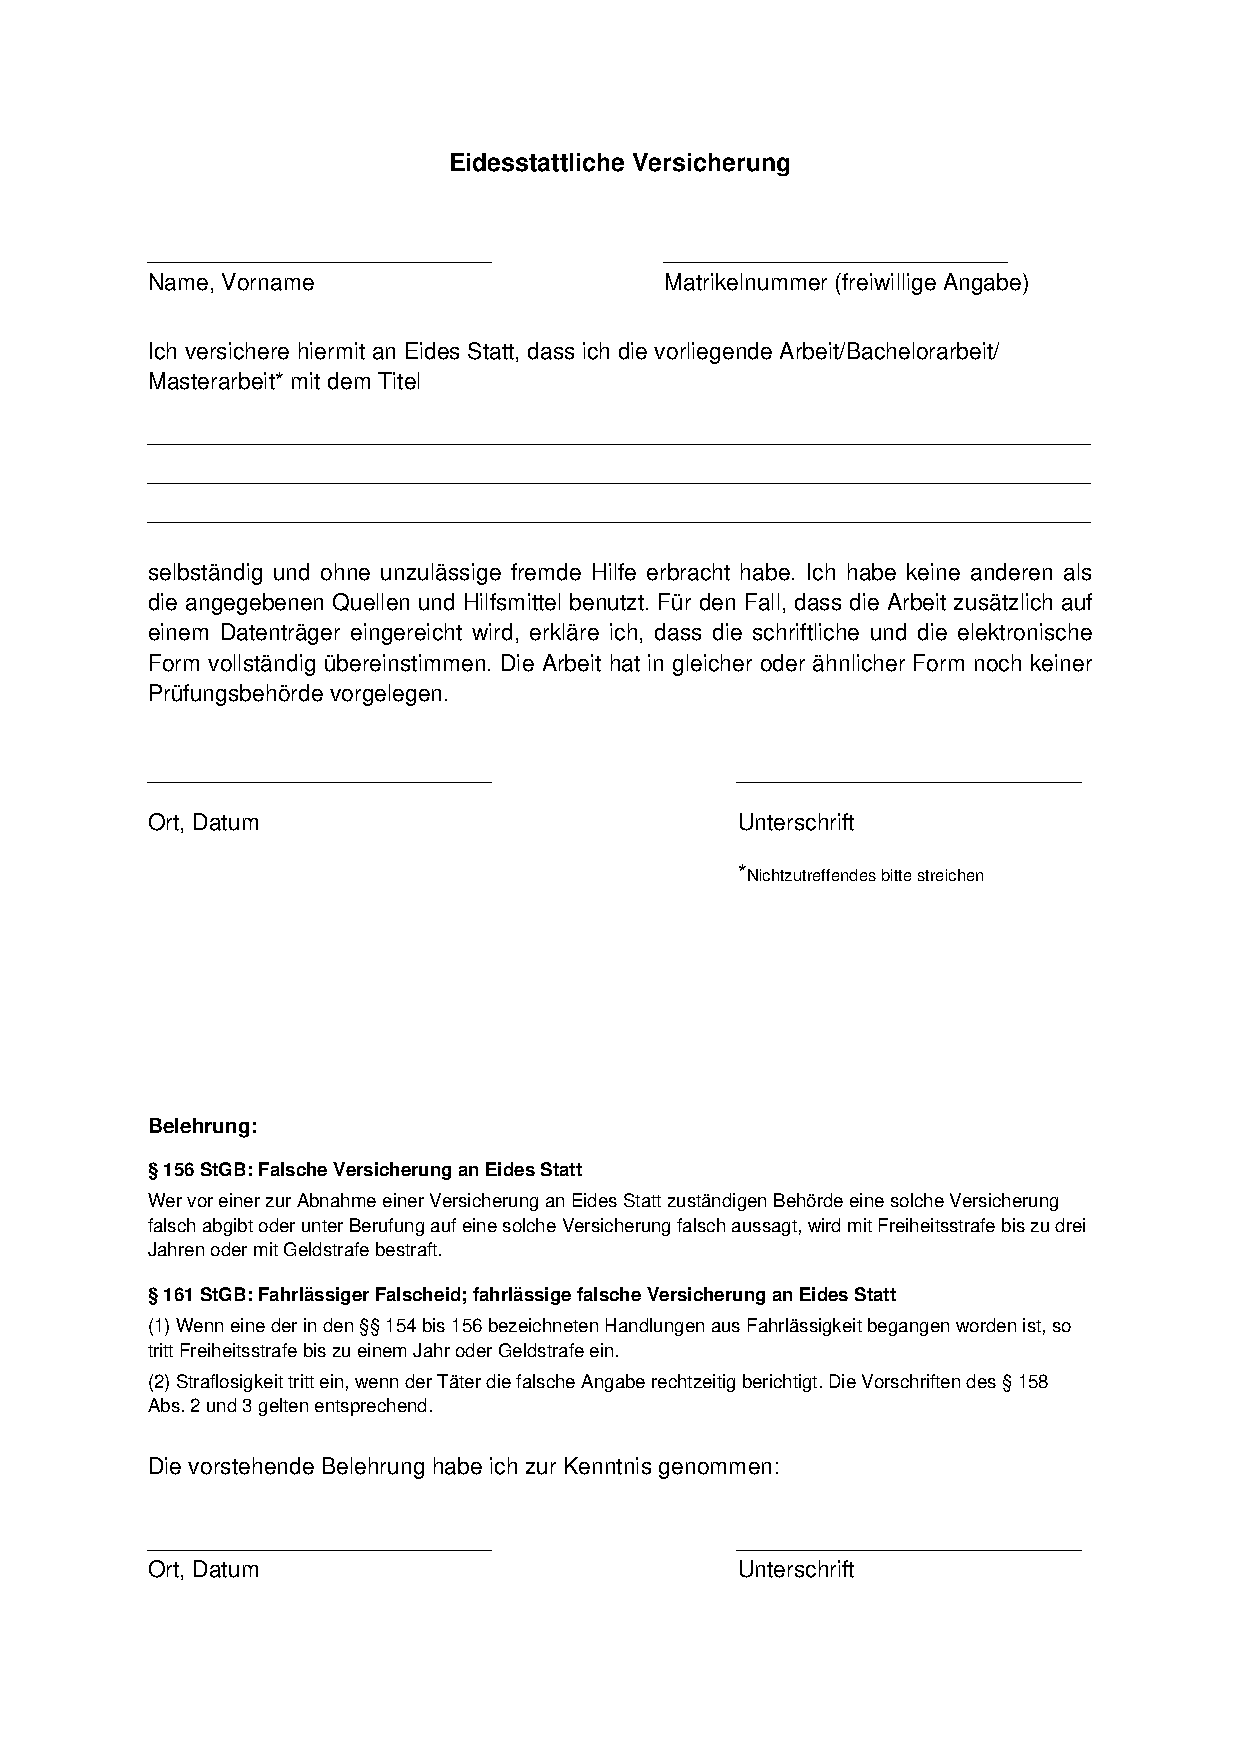
\includepdf{oath.pdf}


\null
\thispagestyle{empty}
\newpage


\begin{center}
\begin{minipage}[t]{0.8\textwidth}
	\section*{Abstract}
We present a semantics for a probabilistic programming language with program variables that can have values in the integers.
The semantics is based on formal power series and is an extension to previous work of Scherbaum~\cite{clara:pgf}.
Scherbaum's semantics does not allow program variables to have negative valuations.
We define a semantic rule for each of the operations in the programming language.
Loops are the most intricate operations.
To ease finding a loop's semantics, we introduce a novel concept to obtain a statement about the semantics of a loop.
It uses binary relations to either find the actual loop semantics or prove an overapproximation of the loop semantics.
An element of such a relation is a pair of input and output of a loop.
Later on, we prove that our semantics is equivalent in expectation to an already established one.
For the comparison, we chose the weakest preexpectation semantics introduced by McIver and Morgan.
We prove that the execution of a program in either semantics gives the same expected value for an arbitrary property expressed as a function over the program variables.
\end{minipage}
\end{center}

\newpage


\tableofcontents
\newpage


\section{Introduction}
Probabilistic programs are programs that do not always produce the same result for one set of inputs.
This is achieved by the usage of probabilistic operations, which are embedded into the programming language itself.
%Contrary to randomised programs, probabilistic programs do not rely on an external source of randomness, but use this inherent mechanism to make random decisions.
Applications are in testing, where error rates can be modelled easily using probabilistic programs.
They can also be used to solve problems that are very hard to solve or are not solvable at all using classical programming paradigms \cite{motwani:randomized}. \\
Because of its non-deterministic nature, code written by using a probabilistic programming language is not easily verified just by reading and understanding.
To obtain insights about properties such as correctness and termination probability, a formal method is necessary.
It should allow to derive statements about the aforementioned properties.
Unlike program code, which describes how something is calculated, the formal method must keep track of what happens while a program is executed.
What happens, or the meaning of the process, is called the program's semantics.
One idea to define a semantics is to keep track of all possible variable valuations, called the program states. \\
Probabilistic programs are not deterministic.
Consequently, program states only have a probability of appearing as result of the whole computation.
To capture all program states with their probabilities, \emph{probability generating functions} (PGFs) can be used.
This thesis is built on work of Scherbaum \cite{clara:pgf}, which uses \emph{formal power series} as PGFs.
These PGFs lack the possibility of having variables with negative values.
Thus, even simple programs that use subtraction cannot be represented by one of those PGFs.
In this work, we will extend Scherbaum's model, so that variables can also have negative values.
Later, we will show that the newly derived semantics is equivalent to an already established one which was introduced by McIver and Morgan.~\cite{mciver:abstraction_refinement}.

\newpage


\section{Preliminaries}
\subsection{Formal Power Series}
A formal power series (FPS) \cite{wilf:generatingfunctionology} is a polynomial of degree $\infty$ over one variable, most commonly $X$.
A formal power series $F$ is an object of the form
\[ F = a_0 X^0 + a_1 \cdot X^1 + a_2 X^2 + \ldots = \infsum a_i X^i \]
The coefficients $a_i$ are real numbers.
When dealing with a formal power series $F$, $F$ is not meant to be a function.
This means that $X$ is not necessarily substituted by a value, so properties like convergence are ignored. \\
Formal power series can be added and multiplied.
Addition comes in a very natural way, it is done componentwise:
\[ F + G = \infsum a_i X^i + \infsum b_i X^i
	= \infsum (a_i + b_i) X^i \]
Multiplication is more complicated.
\[ F \cdot G = \infsum c_i X^i \where c_i = \sum_{k = 0}^{i} a_k b_{i-k} \]
The product of two formal power series is always defined because the sum of every coefficient $c_i$ consists of only finitely many elements.
In fact, the formal power series form a ring under addition and multiplication.
The ring's additive and multiplicative identities are
\[ 0 = \infsum 0 X^i \text{ and } 1 = 1 X^0 + 0 X^1 + 0 X^2 + \ldots \]
Later on, we will need another operation on formal power series, the scalar multiplication:
\[ \alpha \cdot F = \infsum (\alpha \cdot a_i) X^i \where \alpha \in \R \]
Obviously, scalar multiplication always has a formal power series as its result.
Some formal power series even have a closed form.
A closed form is desirable because it eases readability and calculation.
As an example, let us have a look at the geometric series.
It comes up often and is defined as follows:
\[ G = 1 X^0 + p X^1 + p^2 X^2 + \ldots = \infsum p^i X^i \where |p| < 1 \]
The closed form of this series is
\[ G = \frac{1}{1 - pX} \]
This means that $1 - pX$ is the multiplicative inverse of $G$.
In other words: $G \cdot (1 - pX) = 1$ where 1 on the right hand side is the identity of the ring, as given above.
In fact, the equation also holds if $|p| > 1$ because we do not consider convergence of the sums.
$|p| < 1$ must only hold if we want to call a PGF a geometric series.

\subsubsection*{Absolute Value}
Despite ignoring convergence etc.\ during operations on formal power series, it is sometimes useful to know about the sum of all coefficients.
Summing all coefficients is comparable to substituting the formal variable $X$ with 1, or evaluating the series at 1.
It may happen that the sum diverges, but when it does not, it can have a meaningful interpretation as we will see later.
Given a formal power series $G = \infsum a_i X^i$, define the absolute value $|G|$ as the sum of all its coefficients:
\[ |G| = \infsum a_i \]
Here, we have another reason why closed forms of formal power series are interesting.
Consider the geometric series
\[ G = \infsum \half^i X^i \]
Now, calculate the absolute value of both the closed and non closed form.
\begin{align*}
	|G| &= \l| \infsum \half^i X^i \r| = \infsum \half^i = 2 \\
	\\
	|G| &= \l| \frac{1}{1 - \frac{1}{2} X} \r| = \frac{1}{1 - \frac{1}{2}} = 2
\end{align*}
Of course, they both have the same value because they are equivalent.
Nonetheless, calculating the absolute value of the closed form is easier, since fractional arithmetic is simpler than reasoning about the value of a series. \\
Note that, although the notation may suggest it, the absolute value is \emph{not} a norm in the classical sense.
It is rather a linear function because the following holds:
\[ |a \cdot G + F| = a \cdot |G| + |F| \]

\subsection{Multivariate Formal Power Series}
Multivariate formal power series are similar to formal power series except they can have more than one formal variable.
A multivariate formal power series $G$ is an object of the form
\[ G = \multisum{a_s} \where k \in \N_{> 0} \]
Addition is defined componentwise as it is for formal power series.
\[ F + G = \multisum{a_s} + \multisum{b_s} = \multisum{(a_s + b_s)} \]
Multiplication again is more complicated, but is defined in a similar fashion as for formal power series.
\begin{align*}
	& F \cdot G = \multisum{c_s} \\
	& \text{where } c_s = \sum_{\substack{n \in \N^k \land \\
		n_j \leq s_j \text{ for all } j \in \{1,\dots,k\}}}
		a_{n_1, \dots, n_k} \cdot b_{s_1 - n_1, \dots, s_k - n_k}
\end{align*}
The concepts of scalar multiplication and absolute value are defined as expected for multivariate formal power series.

\subsection{Formal Power Series As Probability Generating Functions}
We mentioned earlier that formal power series can be used as probability generating functions.
Given a formal power series
\[ G = \multisum{\mu_s} \]
$\mu_s$ is interpreted as the probability that the random variables $X_1, \ldots, X_k$ have the values $s_1, \ldots, s_k$. In other words
\[ \mathcal{P}(X_1 = s_1, \ldots, X_k = s_k) = \mu_s \]
When used as PGFs, formal power series can still be added, scaled and multiplied.

\subsection{Programs}
In order to reason about probabilistic programs by means of a semantics, we need to define a programming language.
We will use the same language as in \cite{clara:pgf}.
It consists of seven different operations that can be combined to form programs.

\subsubsection*{Basic Operations}
\begin{enumerate}
	\item $\nop$ \vspace{0.3\baselineskip} \\
		The $\nop$ operation does nothing and simply goes on to the next operation.
		It is useful in composite operations.
	\item $\abort$ \vspace{0.3\baselineskip} \\
		The $\abort$ operation does not terminate.
	\item ${X := e}$ \vspace{0.3\baselineskip} \\
		The variable $X$ is assigned the value of $e$.
		$e$ is an expression over the program variables that is evaluated right before the assignment to $X$.
\end{enumerate}
\subsubsection*{Composite Operations}
Here, $P, P_1$ and $P_2$ are programs and $B$ is a Boolean condition.
\begin{enumerate}
	\item ${P_1; P_2}$ \vspace{0.3\baselineskip} \\
		The concatenation $P_1; P_2$ means to first execute $P_1$ and then $P_2$.
	\item $\ifp{B}{P_1}{P_2}$ \vspace{0.3\baselineskip} \\
		If the current variable valuations satisfy the condition $B$ then $P_1$ is executed, otherwise $P_2$ is executed.
	\item $\{P_1\}[p]\{P_2\}$ for some $p \in [0, 1]$ \vspace{0.3\baselineskip} \\
		This statement is called probabilistic choice and is what distinguishes this programming language from classical ones.
		Either $P_1$ or $P_2$ is executed at random.
		$P_1$ is executed with probability $p$ and $P_2$ is executed with probability $1-p$.
	\item $\while{B}{P}$ \vspace{0.3\baselineskip} \\
		The \emph{loop body} $P$ is repeatedly executed until the \emph{loop condition} $B$ is no longer satisfied by the program variables.
\end{enumerate}

\subsection{PGF Semantics}
In \cite{clara:pgf}, a semantics for probabilistic programs with multivariate power series as probability generating functions is introduced.
In the following, let $P$ be a program and $G$ be a PGF with
\[ G = \multisum{\mu_s} \]
where $k$ is equal to the number of program variables used in $P$. \\
Every element of the sum in $G$ corresponds to one possible program state with its probability of occurrence.
For example \[ \frac{1}{3} X_1^2 X_2^5 \] means that with probability $\frac{1}{3}$, variable $X_1$ has value 2 and variable $X_2$ has value 5.
It is easy to see that the absolute value $|G|$ must be less than or equal to 1, because otherwise the total probability of all program states would be greater than 1.
% $|G|$ is also the probability that a program terminates.
Note that the sum of a PGF ranges over $\N^k$, so a variable cannot have a negative value.
Assignments or rather expressions are constrained to only evaluate to positive values. \\
Every $P$ has a corresponding function, denoted by $\smtx{P}$, that transforms an initial PGF into the PGF that results from executing $P$.
These functions are defined next.
\subsubsection*{Basic Operations}
\begin{enumerate}
	\item $\smtx{\nop}(G) = G$
	\item $\smtx{\abort}(G) = 0 = \multisum{0}$
	\item $\smtx{X_j := e}(G) = \sum\limits_{s \in \N^k} \mu_s X_1^{s_1} \cdots X_j^{e(s)} \cdots X_k^{s_k}$
	\item
	$\resP{G} = \sum\limits_{s \in \N^k} \begin{cases}
	\mu_s X_1^{s_1} \cdots X_k^{s_k} &\text{if } s \models B \\
	0 & \text{otherwise}
	\end{cases}$ \\
	\\
	\item[] Above, $s$ is an element of $\N^k$.
	$s_j$ refers to the $j$th components of $s$.
	Of course, $1 \leq j \leq k$.
\end{enumerate}
\subsubsection*{Composite Operations}
Here, $P,\ P_1$, and $P_2$ are programs and $B$ is a Boolean condition.
\begin{enumerate}
	\item $\smtx{P_1; P_2}(G) = \smtx{P_2}( \smtx{P_1}(G) )$
	\item $\smtx{ \{P_1\}[p]\{P_2\} }(G) = p \cdot \smtx{P_1}(G) + (1-p) \cdot \smtx{P_2}(G)$
	\item $\smtx{\ifp{B}{P_1}{P_2}}(G) = \smtx{P_1}(\resP{G}) + \smtx{P_2}(\resN{G})$
	\item $\smtx{\while{B}{P}}(G) = \sup\limits_{n \in \N}
		\l\{ \resN{\operatorname{H}_{P, B}^n(G)} \r\}
		\where \operatorname{H}_{P, B}(G) = \smtx{P}(\resP{G}) + \resN{G}$ \\
		$\operatorname{H}_{P, B}$ represents a single iteration of the loop body.
\end{enumerate}
Similar to how programs are concatenated to form longer programs, their individual semantics functions are composed to form the semantics function of the longer program. \\
If $G'$ results from executing a program $P$ on an initial PGF $G$, i.e. $G' = \smtx{P}(G)$, then $|G'|$ is the termination probability of $P$ given the initial distribution.
A simple example is $\abort$.
Applying $\abort$ to any PGF always results in 0, which has absolute value 0, meaning its termination probability is 0.
This is exactly how $\abort$ is defined.
Later, we will see loops that have a termination probability of less than 1.
\newpage


\section{Extended Semantics}
\begin{frame}
	\frametitle{Challenges}
	\begin{itemize}
		\itemspacing{20pt}
		\item<1-> Extension to negative variable valuations
		\item<2-> Use formal power series
		\item<3-> Usage of closed forms (requires a ring)
	\end{itemize}
\end{frame}

\begin{frame}
	\frametitle{Extended PGFs}
	\begin{itemize}[<+->]
		\itemspacing{20pt}
		\item $ \sum\limits_{s \in \alert<+>{\N^k} } \mu_s \Xok $
		\item $ \sum\limits_{s \in \alert<.>{\Z^k} } \mu_s \Xok $
		\item No ring, no closed forms.
		\item Solution: Use PGFs for partitions of the state space.
	\end{itemize}
\end{frame}

\begin{frame}
	\frametitle{Partitions}
	\begin{columns}
		\begin{column}{0.5\textwidth}
			\begin{itemize}
				\itemspacing{10pt}
				\item<1-> One variable X
				\item<2-> State space is $\Z$.
				\item<3-> Partitions are \\
					$\phantom{-}\N$ \\
					$-\N_{> 0}$ \\
					$\phantom{\N}$ \\ % empty lines for alignment with second column
					$\phantom{\N}$
			\end{itemize}
		\end{column}
		\begin{column}{0.5\textwidth}
			\begin{itemize}
				\itemspacing{10pt}
				\item<4-> Two variables X, Y
				\item<5-> State space is $\Z^2$.
				\item<6-> Partitions are \\
					$\phantom{-}\N_{\phantom{> 0}} \times \phantom{-}\N  $  \\
					$          -\N_{> 0}				   \times \phantom{-}\N  $  \\
					$\phantom{-}\N_{\phantom{> 0}} \times           -\N_{> 0}$  \\
					$          -\N_{> 0}				   \times           -\N_{> 0}$
			\end{itemize}
		\end{column}
	\end{columns}
\end{frame}

\begin{frame}
	\frametitle{Partitions}
	\begin{itemize}[<+->]
		\item $ S_1, S_2, \ldots, S_{2^k} $
		\item $ \sum\limits_{s \in \alert<.>{S_1}} \mu_s \Xok, $ \\[10pt]
			\uncover<+->{
					$ \sum\limits_{s \in \alert<.>{S_2}} \mu_s \Xok, $ \\[10pt]
			}
			\uncover<+->{
					$ \vdots $ \\[10pt]
					$ \sum\limits_{s \in \alert<.>{S_{2^k}}} \mu_s \Xok $
			}
	\end{itemize}
\end{frame}

\begin{frame}
	\frametitle{Semantic Tuples}
	\begin{definition}[Semantic Tuple]
		Let $P$ be a program of $k$ variables.
		A \emph{semantic tuple} $T_G$ is an object of the form
		\[ T_G = \l( \sum_{s \in \alert<1>{S_1}} \mu_s \Xok, \ldots,
		\sum_{s \in \alert<1>{S_{2^k}}} \mu_s \Xok \r) \]
	\end{definition}
	\begin{itemize}
		\itemspacing{10pt}
		\item<2-> Number of entries grows exponentially.
		\item<3-> Use extended PGFs: $ \sum\limits_{s \in \Z^k} \mu_s \Xok $
	\end{itemize}
\end{frame}

\begin{frame}
	\frametitle{PGF Semantics}
	\begin{itemize}[<+->]
		\itemspacing{20pt}
		\item $\smtx{\nop}(G) = G$
		\item $\smtx{\abort}(G) = 0$
		\item $\smtx{X_j := e}(G) = \sum\limits_{s \in \Z^k} \mu_s X_1^{s_1}
		\cdots X_j^{ \alert<+>{ e(s) } } \cdots X_k^{s_k}$
		\item $\resP{G} = \sum\limits_{s \in \Z^k} \begin{cases}
				\mu_s X_1^{s_1} \cdots X_k^{s_k} &\text{if } s \models B \\
				0 & \text{otherwise}
			\end{cases}$
		\item $ \res{0.4 X^1 Y^0 + 0.6 X^4 Y^4}{X = 1} = 0.4 X^1 Y^0 $
	\end{itemize}
\end{frame}

\begin{frame}
	\frametitle{PGF Semantics}
	\begin{itemize}[<+->]
		\itemspacing{20pt}
		\item $\smtx{P_1; P_2}(G) = \smtx{P_2}( \smtx{P_1}(G) )$
		\item $\smtx{ \{P_1\}[p]\{P_2\} }(G) = p \cdot \smtx{P_1}(G) + (1-p) \cdot \smtx{P_2}(G)$
		\item $\smtx{\ifp{B}{P_1}{P_2}}(G) = \smtx{P_1}(\resP{G}) + \smtx{P_2}(\resN{G})$
		\item $ \smtx{\while{B}{P}}(G) $
%			= \sum\limits_{i = 0}^{\infty} \resN{\wh^i(G)} $
%		\item $ \wh(G) = \smtx{P}(\resP{G}) $
	\end{itemize}
\end{frame}

\begin{frame}
	\frametitle{Loop semantics}
	\begin{itemize}[<+->]
		\itemspacing{10pt}
		\item $ \wh(G) = \smtx{P}(\resP{G}) $
		\item $ \wh^{\alert<.>{n}}(G) $ is the $n$th loop iteration.
		\item $ \alert<.(1)>{ \resN{ \wh^{n}(G) } } $ drops out after $n$ iterations.
		\item $ \smtx{\while{B}{P}}(G)
			= \sum\limits_{i = 0}^{\infty} \alert<.>{ \resN{\wh^i(G)} } $
	\end{itemize}
\end{frame}
\newpage


\section{Case Studies}
\begin{frame}[fragile]
	\frametitle{Canonical Example}
	\begin{lstlisting}
 while ( F = 0 ) {
   { X := X - 1 }[0.5]{ F := 1 }
 }
	\end{lstlisting}
	\begin{itemize}
		\itemspacing{10pt}
		\item<2-> $ \smtx{\while{B}{P}}(G) = 
			\sum\limits_{i = 0}^{\infty} \alert<3>{ \resN{\wh^i(G)} } $
		\item<4-> $ B = (F = 0) $
		\item<5-> $ P = \{ X := X - 1 \}[0.5]\{ F := 1 \} $
		\item<6-> $ G = 1 X^0 F^0 = 1 $
	\end{itemize}
\end{frame}

\begin{frame}
	\frametitle{Canonical Example}
	\begin{itemize}[<+->]
		\itemspacing{10pt}
		\item $ \resN{\wh^1(1)} = \hf X^0 F^1 $
		\item $ \resN{\wh^2(1)} = \qu X^{-1} F^1 $
%		\item $ \ldots $
		\item $\resN{\wh^n(1)} = \half^n X^{-(n-1)} F^1 $
		\item $ \sum\limits_{i = 0}^{\infty} \resN{\wh^i(G)}
			= \alert<.>{\hf \cdot \sum\limits_{i = 0}^{\infty} \half^i X^{-i} F^1} $
		\item Closed form: $ \frac{F}{2 - X^{-1}} $
		\item Actually: $ \pair{0, \frac{F}{2 - X^{-1}}, 0, 0} $
	\end{itemize}
\end{frame}

\begin{frame}[fragile]
\frametitle{Termination Probability}
\begin{lstlisting}
while ( F = 0 ) {
  {
    { X := X + 1 }[0.5]{ diverge }
  }[0.5]{
    F := 1
  }
}
\end{lstlisting}
\begin{itemize}[<+(1)->]
	\itemspacing{10pt}
	\item $ \resN{\wh^i \l(G\r)} = \hf \cdot \l(\frac{1}{4}\r)^{i-1} X^{i-1} F^1 $
	\item $ \sum\limits_{i = 0}^{\infty} \resN{\wh^i(G)}
	= \alert{\hf \cdot \sum\limits_{i = 0}^{\infty} \l(\frac{1}{4}\r)^i X^i F^1} $
\end{itemize}
\end{frame}

\begin{frame}
	\frametitle{Termination Probability}
	\begin{itemize}[<+->]
		\itemspacing{10pt}
		
		\item Closed form: $ \frac{F}{2 - \hf X} $
		\item Termination probability using absolute value:
		\item $ \l| \hf \cdot \sum\limits_{i = 0}^{\infty} \l(\frac{1}{4}\r)^i X^i F^1 \r|
			\uncover<+->{
				= \hf \cdot \sum\limits_{i = 0}^{\infty} \l(\frac{1}{4}\r)^i 
			}
			\uncover<+->{
				=  \frac{2}{3}
			} $
		\item $ \l| \frac{F}{2 - \hf X} \r| = \frac{1}{2 - \hf} = \frac{2}{3} $
	\end{itemize}
\end{frame}

\begin{frame}[fragile]
	\frametitle{Equivalent Programs}
	\begin{columns}
		\begin{column}[t]{0.5\textwidth}
			\begin{lstlisting}[basicstyle=\scriptsize]
while ( F = 0 ) {
  { X := X + 1 }[p]{ F := 1 }
};
 
F := 0;
while ( F = 0 ) {
  { X := X - 1 }[q]{ F := 1 }
}
			\end{lstlisting}
		\end{column}
		\hspace{-20pt}
		{ \vrule width 1pt }
%		\vrule{}
		\hspace{7pt}
		\begin{column}[t]{0.5\textwidth}
			\begin{lstlisting}[basicstyle=\scriptsize]
{ F := 0 }[0.5]{ F := 1 };
if ( F = 0 ) {
  while ( F = 0 ) {
    { X := X + 1 }[p]{ F := 1 }
  }

} else {
  F := 0;
  while ( F = 0 ) {
    X := X - 1;
    { skip }[q]{ F := 1 }
  }
}
			\end{lstlisting}
		\end{column}
	\end{columns}
\end{frame}

\begin{frame}[fragile]
	\frametitle{Equivalent Programs}
	\begin{columns}
		\begin{column}[t]{0.5\textwidth}
			\begin{lstlisting}[basicstyle=\tiny]
while ( F = 0 ) {
  { X := X + 1 }[p]{ F := 1 }
};

F := 0;
while ( F = 0 ) {
  { X := X - 1 }[q]{ F := 1 }
}
			\end{lstlisting}
		\end{column}
		\begin{column}[t]{0.5\textwidth}
			\begin{lstlisting}[basicstyle=\tiny]
{ F := 0 }[0.5]{ F := 1 };
if ( F = 0 ) {
  while ( F = 0 ) {
    { X := X + 1 }[p]{ F := 1 }
  }

} else {
  F := 0;
  while ( F = 0 ) {
    X := X - 1;
    { skip }[q]{ F := 1 }
  }
}
			\end{lstlisting}
		\end{column}
	\end{columns}
	\begin{itemize}[<+->]
		\item Introduced by Kiefer et al. in 2012.
		\item Proven equivalent in distribution for $p = \frac{1}{2}$ and $q = \frac{2}{3}$.
		\item Expected value of $X$ is the same if $q = \frac{1}{2-p}$. (Gretz et al.)
		\item Today: equivalence in distribution if $q = \frac{1}{2-p}$.
	\end{itemize}
\end{frame}

\begin{frame}
	\frametitle{Equivalent Programs}
	\begin{itemize}[<+->]
		\item First program's semantics: \\[10pt]
			$ \alert<.(4)>{ \frac{(1-q) \cdot (1-p)}{1-qp} } \cdot	% factor
			\pair{
				\alert<.(2)>{ \frac{F}{1 - p X} }, \ % first entry sum
				\alert<.(4)>{ q } \cdot	% second entry factor
					\alert<.(3)>{ \frac{X^{-1} F}{1 - q X^{-1}} } % snd entry sum
				, 0, 0 % null entries
			} $
			\vspace*{20pt}
		\item Second program's semantics: \\[10pt]
			$ \pair{
				\alert<.(3)>{ \frac{1-p}{2} } \cdot	% first entry factor
					\alert<.(1)>{ \frac{F}{1 - p X} }, \ % first entry sum
				\alert<.(3)>{ \frac{1-q}{2} } \cdot	% second entry factor
					\alert<.(2)>{ \frac{X^{-1} F}{1 - q X^{-1}} } % snd entry sum
					, 0, 0 % null entries
			} $
			\vspace*{20pt}
		\item<+(3)-> Solve $ \frac{(1-q) \cdot (1-p)}{1-qp} = \frac{1-p}{2} $ and
			$ \frac{(1-q) \cdot (1-p) \cdot q}{1-qp} = \frac{1-q}{2} $.
			\vspace*{10pt}
		\item<+(3)-> Equivalent in distribution if $ q = \frac{1}{2 - p}$.
	\end{itemize}
\end{frame}

\newpage


\section{Bisimulations}
\begin{frame}
	\frametitle{Bisimulations}
	\begin{itemize}[<+->]
		\itemspacing{20pt}
		\item Inspired by coinduction (Arbab et al.)
		\item Use bisimulations to reason about loops.
    \item Weak and strong bisimulations
    \item No correlation to transition systems
    \item Overapproximation and actual loop semantics
	\end{itemize}
\end{frame}

\begin{frame}
	\frametitle{Bisimulations}
	\begin{center}
		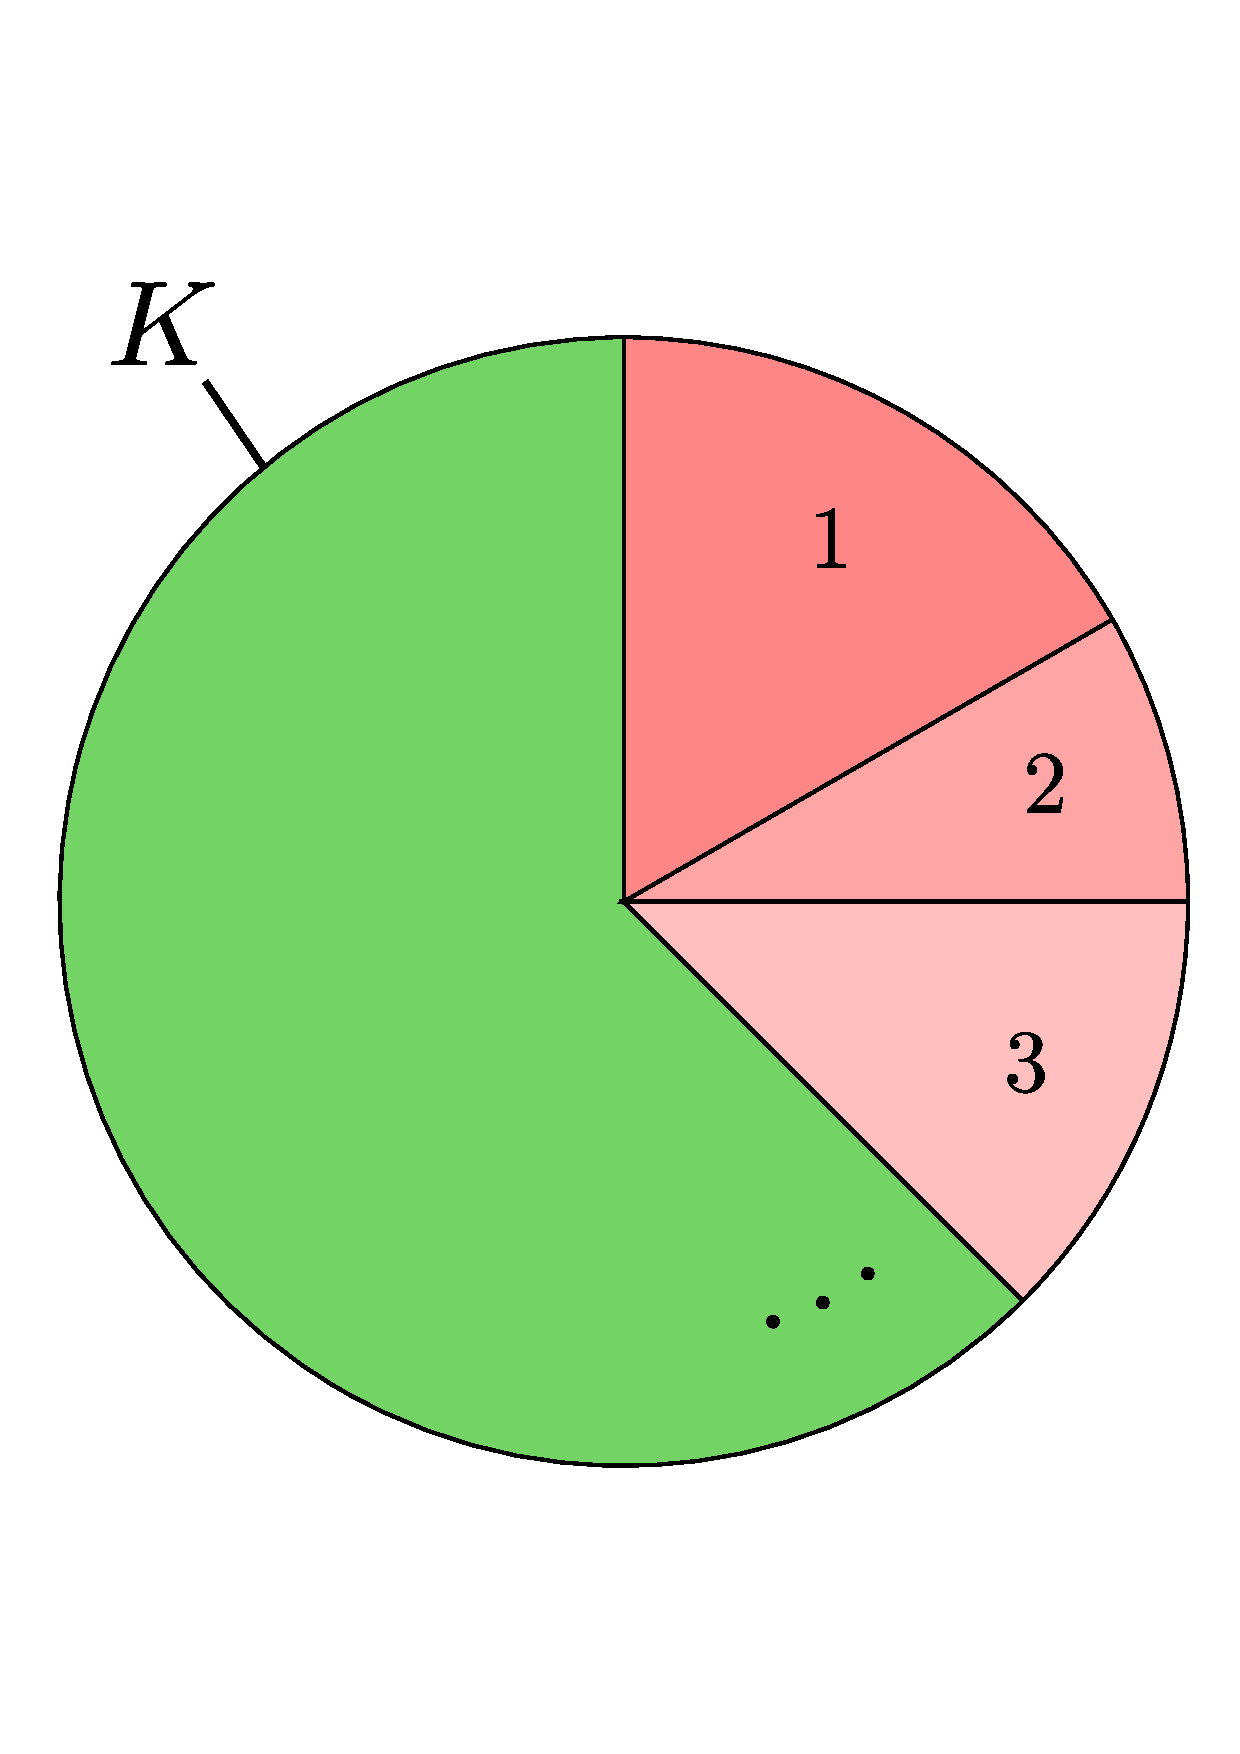
\includegraphics[height=\textheight]{semantics/img/weak_bisimulation.pdf}
	\end{center}
\end{frame}

\begin{frame}
	\frametitle{Bisimulations}
	\uncover<+->{
		\begin{definition}[Weak Bisimulation]
			Let $R$ be a binary relation.
			If $\pair{K, G} \in R$, then
			\begin{enumerate}[i)]
				\itemspacing{7pt}
				\item[] Let $G' = \wh(G)$
				\item $\resN{G'} \sqsubseteq K$
				\item $\pair{K - \resN{G'}, G'} \in R$
			\end{enumerate}
		\end{definition}
	}
	\uncover<+->{
		\begin{theorem}
			Let $R$ be a weak bisimulation.
			Then \[ \pair{K, G} \in R \land G \models B
			\implies \smtx{\while{B}{P}}(G) \sqsubseteq K \]
		\end{theorem}
	}
\end{frame}

\begin{frame}
	\frametitle{Bisimulations}
	\begin{center}
		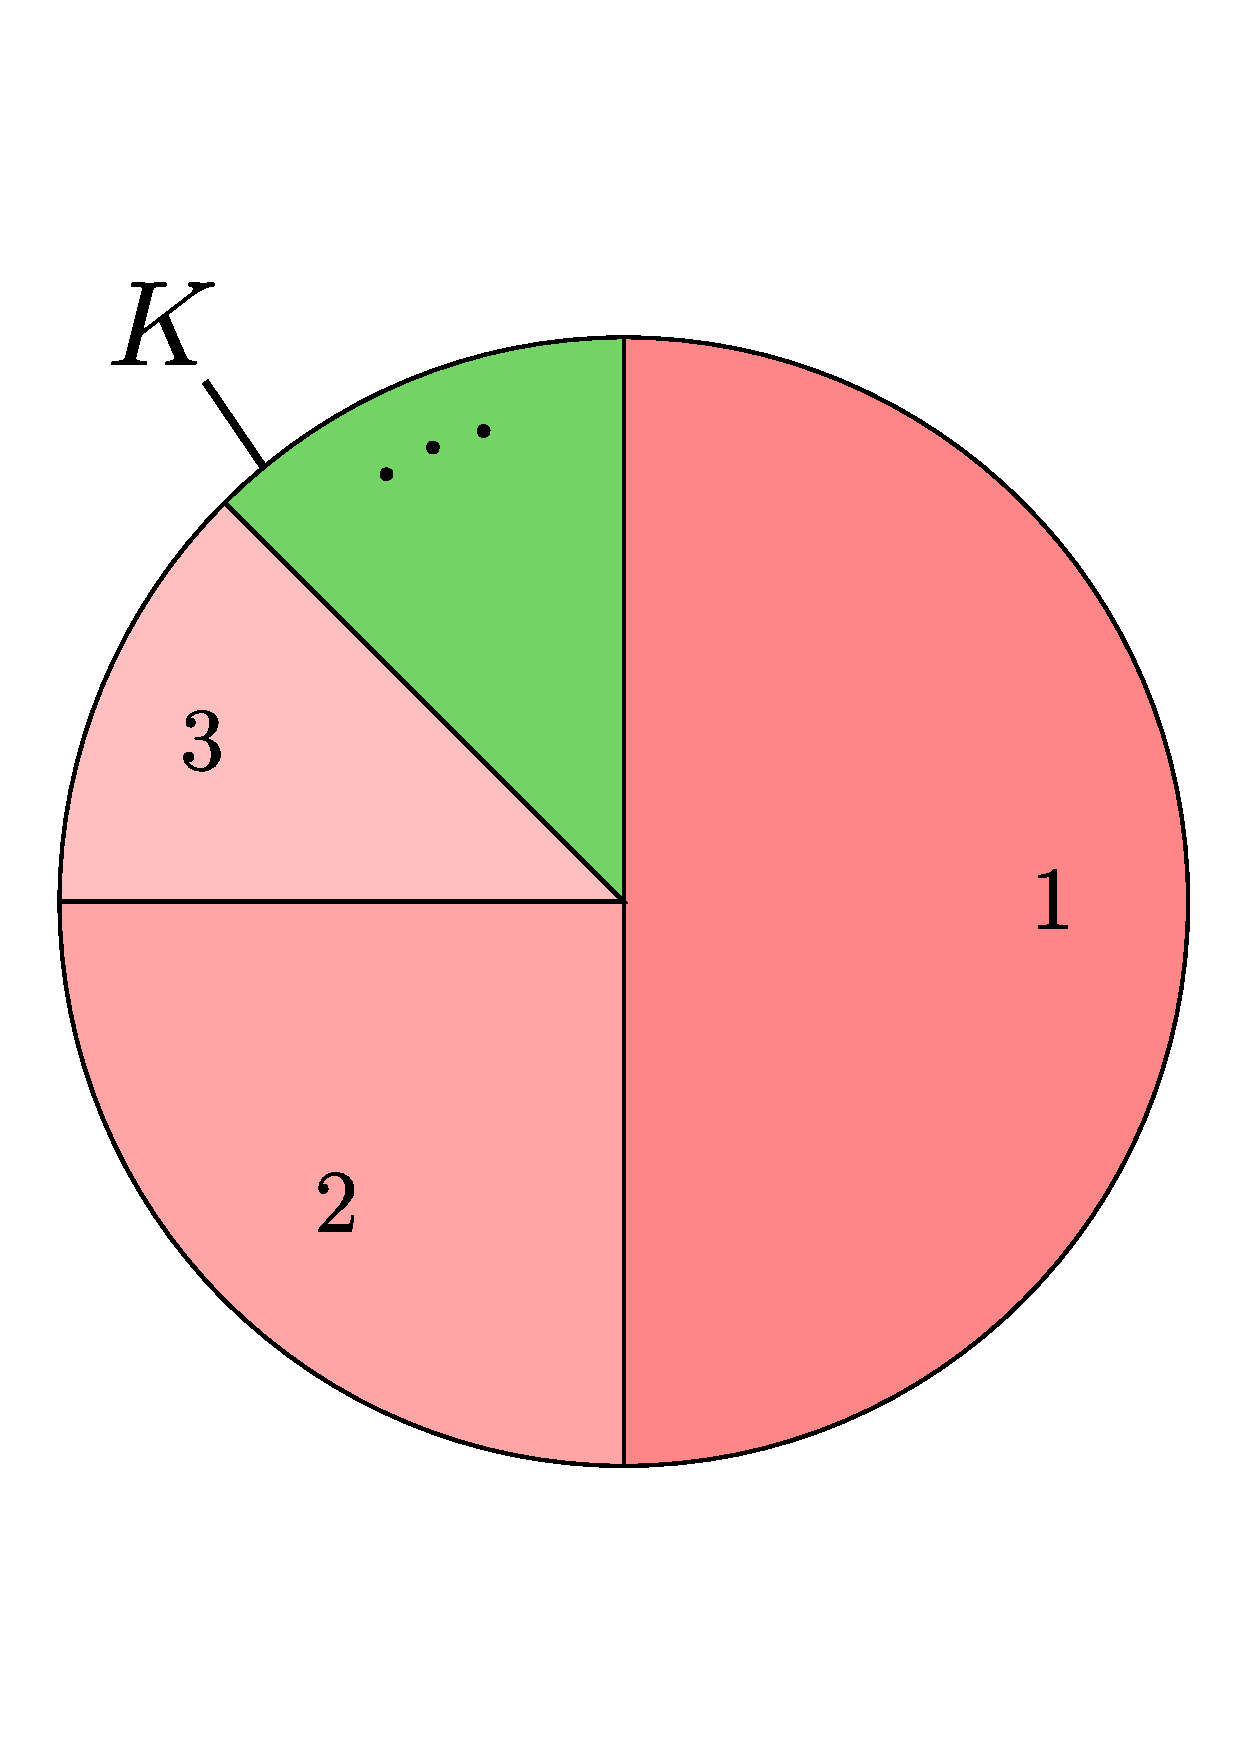
\includegraphics[height=\textheight]{semantics/img/strong_bisimulation.pdf}
	\end{center}
\end{frame}

\begin{frame}
	\frametitle{Bisimulations}
	\uncover<+->{
		\begin{definition}[Strong Bisimulation]
			Let $R$ be a binary relation and $\varepsilon \in (0, 1)$.
			If $\pair{K, G} \in R$, then
			\begin{enumerate}[i)]
				\itemspacing{7pt}
				\item[] Let $G' = \wh(G)$
				\item $\resN{G'} \leqD K$
				\item $\pair{K - \resN{G'}, G'} \in R$
				\item $\left| \resN{G'}\right| \geq \varepsilon \cdot \l| K \r|$
			\end{enumerate}
		\end{definition}
	}
	\uncover<+->{
		\begin{theorem}
			Let $R$ be a strong bisimulation.
			Then \[ \pair{K, G} \in R \land G \models B
				\implies \smtx{\while{B}{P}}(G) = K \]
		\end{theorem}
	}
\end{frame}

\begin{frame}[fragile]
	\frametitle{Bisimulations}
	\begin{lstlisting}
 while (F = 0) {
   {X := X + 1}[0.5]{F := 1}
 }
	\end{lstlisting}
	\begin{itemize}[<+->]
		\itemspacing{10pt}
		\item $ G = 1$, $ K = \frac{1}{2 - X} $
		\item Bisimulation: $ R = \l\{ \pair{K, G}  \r\} \cup
			\only<+->{
				\l\{ \pair{
					\alert<+>{ \res{\frac{1}{2 - X}}{X \geq n} },
					\alert<+>{ \half^n \cdot \l( X^n F^0 + X^{n-1} F^1 \r) } } \ 
					\middle| \ n \in \N_{>0} \r\} 
			} $
		\item $R$ is in fact a strong bisimulation ($\varepsilon = \hf$)!
		\item $ \smtx{\while{F = 0}{\ldots}}(1) \sqsubseteq K $
		\item $ \smtx{\while{F = 0}{\ldots}}(1) = K $
	\end{itemize}
\end{frame}

\newpage


\section{Semantics Equivalence}
\begin{frame}
	\frametitle{Comparison of Semantics}
		\begin{itemize}[<+->]
			\itemspacing{7pt}
			\item Comparison of PGF and wp semantics (McIver and Morgan)
			\item Random variables: $ E = \{ \S \to \R_{\geq 0} \}$
			\item $ \operatorname{wp} \colon P \times E \to E $
			\item $ \smtx{P}(G) $ vs. $ \wp{P, f} $
			\item $ \E_\mu (f) $, where $\mu$ a measure on program states, $f$ a random variable
			\item Every PGF has a corresponding measure.
		\end{itemize}
		\uncover<+->{
			\begin{center}
				\begin{minipage}{0.9\textwidth}
					\begin{theorem}
						Given a program $P$, a measure $\mu$ and an expectation $f$, the following holds:
						\[ \E_{\smtx{P}(\mu)} (f) = \E_\mu (\wp{P, f}) \]
					\end{theorem}
				\end{minipage}
			\end{center}
		}
\end{frame}
\newpage


\section{Conclusion and Future Work}
In this bachelor thesis, we developed a PGF semantics for probabilistic programs with integer program variable valuations.
The semantics is based on semantic tuples which are tuples where each entry is a PGFs.
The number of entries grows exponentially in the number of program variables.
This means that for more than three or four program variables the tuples are hard to handle by hand because they have many entries.
However, with some knowledge about the program we can reduce the number of entries that have to be calculated to find a complete semantic description.
Another way to reduce complexity is to use PGFs with extended range.
Every of these PGFs corresponds to a semantic tuple and can therefore be used as well.
We successfully applied the new semantics to a variety of programs and could even extend the results of Gretz et al.\ concerning two equivalent programs.
We showed that the programs are not only equal in expectation but indeed equal in their semantics.
In the next step, we found a novel approach to prove the semantics of a loop.
Originally, the loop semantics is defined as the sum of all possible loop unrollings.
Now, we can also use binary relations called bisimulations.
A bisimulation is a set of pairs of PGFs.
Each pair is a pair of input and output of the loop that is treated.
There are two types of bisimulations.
Weak bisimulations allow to prove an overapproximation for the loop's semantics.
Strong bisimulations can be used to prove that a pair in the bisimulation is in fact the input and output of the loop.
Last, we showed that our PGF semantics is equivalent in expectation to the weakest preexpectation semantics introduced by McIver and Morgan.
We proved that the execution of a program in either semantics has the same expected value for an arbitrary property expressed as a function over the program variables. \\
In this thesis, we proved that two different programs are equal in their semantics.
Instead of showing equivalence or nonequivalence of two programs, one could find a measure for the similarity of two programs.
This can be done by comparing the semantics of these programs.
In our case, this would require a distance function for PGFs.
Another idea is to find more use cases and other statements that can be derived from weak and strong bisimulations.



\newpage


\section{Appendix}
\subsection{Vector Space of FPSs with Extended Range}
\label{proof:vector_space}
We want to prove that the PGFs with extended range combined with addition and scalar multiplication form a vector space.
Recall the definition of vector space.
\begin{definition}[Vector Space~\cite{brown:vector_space}]
	A vector space $V$ over a field $F$ is a non-empty set $V$ together with two functions, 
	$+ \colon V \times V \to V$ and $\cdot \colon F \times V \to V$,
	which satisfy the following properties:
	\begin{enumerate}
		\item[] Let $u, v, w \in V$ and $r, s \in F$ be arbitrarily chosen.
		\item $ v + w = w + v $
		\item $ u + (v + w) = (u + v) + w $
		\item There exists $0 \in V$ such that $ 0 + v = v  $.
		\item There exists $(-v) \in V$ such that $ v + (-v) = 0 $.
		\item $ (r \cdot s) \cdot v = r \cdot (s \cdot v) $
		\item $ r \cdot (u + v) = r \cdot u + r \cdot v $
		\item $ (r + s) \cdot v = r \cdot v + s \cdot v $
		\item $ 1 \cdot v = v $, where $1$ is the multiplicative identity of the field $F$
	\end{enumerate}
\end{definition}
For the PGFs with extended range, we have
\begin{itemize}
	\item $ V = \l\{ \sum_{s \in \Z^k} \mu_s \Xok \middle| \mu_s \in \R \r\} $
	\item $ F = \R $
\end{itemize}
For $v = \sum_{s \in \Z^k} \mu_s \Xok$ and $w = \sum_{s \in \Z^k}\mu_s' \Xok$
and $r \in \R$, the two operations are defined as follows:
\begin{itemize}
	\item $\begin{aligned}[t]
			& + \colon V \times V \to V \\
			& v + w = \sum_{s \in \Z^k} (\mu_s + \mu_s') \Xok
	\end{aligned}$
	\item $\begin{aligned}[t]
			& \cdot \colon \R \times V \to V \\
			& r \cdot v = \sum_{s \in \Z^k} (r \cdot \mu_s) \Xok
		\end{aligned}$
\end{itemize}
To prove that $(V, \cdot, +)$ is a vector space, we have to prove properties $1$ to $8$.
\begin{theorem}[continues=theo:ext:vectorspace]
	The set of FPSs with extended range combined with addition and scalar multiplication forms a \emph{vector space}.
\begin{proof}
	Let $u, v, w \in V$ with their coefficients $\sigma_s, \mu_s$ and $\tau_s$, respectively, be arbitrarily chosen.
	Additionally, let $r, s \in \R$ be arbitrarily chosen.
	\begin{enumerate}
		\item $\begin{aligned}[t]
			 & v + w \\
			=& \sum_{s \in \Z^k} (\mu_s + \tau_s) \Xok \\
			=& \sum_{s \in \Z^k} (\tau_s + \mu_s) \Xok \\
			=& w + v
		\end{aligned}$
		\item $\begin{aligned}[t]
			 & u + (v + w) \\
			=& \sum_{s \in \Z^k} (\sigma_s + (\mu_s + \tau_s)) \Xok \\
			=& \sum_{s \in \Z^k} ((\sigma_s + \mu_s) + \tau_s) \Xok \\
			=& (u + v) + w
		\end{aligned}$
		\item Let $0 = \sum_{s \in \Z^k} 0 \Xok \in V$.
		Then, \vspace{1em} \\
		$\begin{aligned}[t]
			 & 0 + v \\
			=& \sum_{s \in \Z^k} (0 + \mu_s) \Xok \\
			=& \sum_{s \in \Z^k} \mu_s \Xok \\
			=& v
		\end{aligned}$
		\item Let $-v = \sum_{s \in \Z^k} (-\mu_s) \Xok \in V$.
		Then, \vspace{1em} \\
		$\begin{aligned}[t]
			 & v + (-v) \\
			=& \sum_{s \in \Z^k} (\mu_s + (-\mu_s)) \Xok \\
			=& \sum_{s \in \Z^k} 0 \Xok \\
			=& 0
		\end{aligned}$
		\item $\begin{aligned}[t]
			 & (r \cdot s) \cdot v \\
			=& \sum_{s \in \Z^k} ((r \cdot s) \cdot \mu_s) \Xok \\
			=& \sum_{s \in \Z^k} (r \cdot (s \cdot \mu_s)) \Xok \\
			=& r \cdot \sum_{s \in \Z^k} (s \cdot \mu_s) \Xok \\
			=& r \cdot (s \cdot v)
		\end{aligned}$
		\item $\begin{aligned}[t]
			 & r \cdot (v + w) \\
			=& r \cdot \l( \sum_{s \in \Z^k} (\mu_s + \tau_s) \Xok \r) \\
			=& \sum_{s \in \Z^k} (r \cdot (\mu_s + \tau_s)) \Xok \\
			=& \sum_{s \in \Z^k} (r \cdot \mu_s + r \cdot \tau_s) \Xok \\
			=& \sum_{s \in \Z^k} (r \cdot \mu_s) \Xok
				+ \sum_{s \in \Z^k} (r \cdot \tau_s) \Xok \\
			=& r \cdot \sum_{s \in \Z^k} \mu_s \Xok
				+ r \cdot \sum_{s \in \Z^k} \tau_s \Xok \\
			=& r \cdot v + r \cdot w
		\end{aligned}$
		\item $\begin{aligned}[t]
			 & (r + s) \cdot v \\
			=& \sum_{s \in \Z^k} ((r + s) \cdot \mu_s) \Xok \\
			=& \sum_{s \in \Z^k} (r \cdot \mu_s + s \cdot \mu_s) \Xok \\
			=& \sum_{s \in \Z^k} (r \cdot \mu_s) \Xok
				+ \sum_{s \in \Z^k} (s \cdot \mu_s) \Xok \\
			=& r \cdot \sum_{s \in \Z^k} \mu_s \Xok
			+ s \cdot \sum_{s \in \Z^k} \mu_s \Xok \\
			=& r \cdot v + s \cdot v
		\end{aligned}$
		\item $\begin{aligned}[t]
			 & 1 \cdot v \\
			=& \sum_{s \in \Z^k} (1 \cdot \mu_s) \Xok \\
			=& \sum_{s \in \Z^k} \mu_s \Xok \\
			=& v
		\end{aligned}$
	\end{enumerate}
	$(V, \cdot, +)$ satisfies all 8 properties, so it is a vector space.
\end{proof}
\end{theorem}

\subsection{$D$ and $L$ Are $\boldsymbol{\omega}$-Complete Partial Orders}
\label{proof:cpos}
$D_k$ was defined as the set of all PGFs over $k$ variables with its coefficients and absolute value in $[0,1]$.
$L_k$ is the set of all functions mapping $D_k$ to $D_k$.
To show that $D_k$ and $L_k$ are $\omega$-complete partial orders~\cite{winskel:cpos}, we have to show the following:
\begin{enumerate}
	\item $D_k$ and $L_k$ are reflexive.
	\item $D_k$ and $L_k$ are transitive.
	\item $D_k$ and $L_k$ are antisymmetric.
	\item Every $\omega$-chain in $D_k$ or $L_k$ has a supremum.
\end{enumerate}
\begin{lemma}[continues=lem:ext:cpos]
	$D_k$ is an $\omega$-complete partial order for all $k \in \N \setminus \{0\}$.
	\begin{proof}
		In the following, let $r, s$ and $t$ be arbitrary elements in $D_k$ with their coefficients $\rho_i, \sigma_i$ and $\tau_i$ for $i \in \Z^k$.
		\begin{enumerate}
			\item $\forall i \in \Z^k \colon \rho_i \leq \rho_i \iff r \leqD r$
			
			\item Assume $r \leqD s$ and $s \leqD t$.
			Then \begin{align*}
				& \forall i \in \Z^k \colon \rho_i \leq \sigma_i \land
					\forall i \in \Z^k \colon \sigma_i \leq \tau_i \\
				\implies & \forall i \in \Z^k \colon \rho_i \leq \sigma_i
					\land \sigma_i \leq \tau_i \\
				\implies & \forall i \in \Z^k \colon \rho_i \leq \tau_i \\
				\implies & r \leqD t
			\end{align*}
			
			\item Assume $r \leqD s$ and $s \leqD r$.
			Then \begin{align*}
				& \forall i \in \Z^k \colon \rho_i \leq \sigma_i \land
				\forall i \in \Z^k \colon \sigma_i \leq \rho_i \\
				\implies & \forall i \in \Z^k \colon \rho_i \leq \sigma_i
					\land \sigma_i \leq \rho_i \\
				\implies & \forall i \in \Z^k \colon \sigma_i = \rho_i \\
				\implies & r = t
			\end{align*}
			
			\item Note: Because of the  various subscripts, only in this fourth item, we will denote the coefficient of a PGF $G$ corresponding to $i \in \Z^k$ with $G(i)$. \\
			Let $d_1 \leqD d_2 \leqD d_3 \leqD \ldots$ be an $\omega$-chain in $D_k$.
			The coefficients of $d_n$ are now $d_n(i)$ for $i \in \Z^k$.
			The supremum $d_{\sup}$ of the $\omega$-chain is given by
			\[ d_{\sup}
				= \sup_{n \in \N} \{d_n\}
				= \sum_{i \in \Z^k} \sup_{n \in \N}
				\l\{ d_n(i) \r\} X_1^{i_1} \cdots X_k^{i_k} \]
			The supremum $\sup_{n \in \N} \{ d_n(i) \}$ exists because $d_n(i) \leq 1$ for all $i \in \Z^k$ by definition of $D_k$.
			It remains to prove that $d_{\sup}$ is in fact the supremum of the $\omega$-chain.
			\begin{enumerate}[i)]
				\item \textit{$d_{\sup}$ is an upper bound for all $d_n$}. \\
				Assume the contrary.
				Then there is an index $n \in \N$ such that $d_{\sup} \sqsubsetneq_D d_n$.
				Then there exists an $i \in \Z^k$ such that
				$d_n(i) > d_{\sup}(i) = \sup_{n \in \N} \{ d_n(i) \}$.
				This is a contradiction to the definition of supremum, so $d_{\sup}$ is an upper bound for all $d_n$.
				
				\item \textit{There is no $d'$ with $d_n \leqD d' \sqsubsetneq_D d_{\sup}$ for all $n \in \N$}. \\
				Assume $d'$ exists.
				Then there exists $i \in \Z$ such that $d_n(i) \leq d'(i) < d_{\sup}(i) = \sup_{n \in \N} \{ d_n(i) \}$.
				This is a contradiction to the definition of supremum, so $d'$ cannot exist.
			\end{enumerate}
			By the items i) and ii) above, $d_{\sup}$ is the supremum of the $\omega$-chain.
		\end{enumerate}
		All four items above are proven, so $D_k$ is an $\omega$-complete partial order.
	\end{proof}
\end{lemma}

\begin{lemma}
	$L_k$ is an $\omega$-complete partial order for all $\N \setminus \{0\}$.
	\begin{proof}
		In the following, let $f, g$ and $h$ be arbitrary elements in $L_k$.
		\begin{enumerate}
			\item $D_k$ is reflexive, so $\forall d \in D_k \colon f(d) \leqD f(d)
			\iff f \leqL f$.
			
			\item Assume $f \leqL g$ and $g \leqL h$.
			Then \begin{align*}
				& \forall d \in D_k \colon f(d) \leqD g(d) \land
				\forall d \in D_k \colon g(d) \leqD h(d) \\
				\implies & \forall d \in D_k \colon f(d) \leqD g(d) \land g(d) \leqD h(d) \\
				& \explain{$D_k$ is transitive} \\
				\implies & \forall d \in D_k \colon f(d) \leqD h(d) \\
				& \explain{definition of $\leqL$} \\
				\implies & f \leqL h
			\end{align*}
			
			\item Assume $f \leqL g$ and $g \leqL f$.
			Then \begin{align*}
				& \forall d \in D_k \colon f(d) \leqD g(d) \land
				\forall d \in D_k \colon g(d) \leqD f(d) \\
				\implies & \forall d \in D_k \colon f(d) \leqD g(d) \land g(d) \leqD f(d) \\
				& \explain{$D_k$ is antisymmetric} \\
				\implies & \forall d \in D_k \colon f(d) = g(d) \\
				\implies & f = g
			\end{align*}
			
			\item Let $f_1 \leqL f_2 \leqL f_3 \leqL \ldots$ be an $\omega$-chain in $L_k$.
			The supremum $l_{\sup}$ of the $\omega$-chain is given by
			\[ l_{\sup}(d) = \sup_{n \in \N} \{ f_n(d) \} \]
			The supremum on the the right hand side exists because $f_1(d) \leqD f_2(d) \leqD f_3(d) \leqD \ldots$ is an $\omega$-chain in $D_k$ for every $d \in D_k$.
			It remains to prove that $l_{\sup}$ is in fact the supremum of the $\omega$-chain.
			\begin{enumerate}[i)]
				\item \textit{$f_{\sup}$ is an upper bound for all $f_n$}. \\
				Assume the contrary.
				Then there is an index $n \in \N$ such that $f_{\sup} \sqsubsetneq_L f_n$.
				Then there exists a $d \in D_k$ such that
				$f_n(d) \sqsupsetneq_L f_{\sup}(d) = \sup_{n \in \N} \{ f_n(d) \}$.
				This is a contradiction to the definition of supremum, so $f_{\sup}$ is an upper bound for all $f_n$.
				
				\item \textit{There is no $f'$ with $f_n \leqL f' \sqsubsetneq_L f_{\sup}$ for all $n \in \N$}. \\
				Assume $f'$ exists.
				Then there exists $d \in D_k$ such that $f_n(d) \leqD f'(d) \sqsubsetneq_D f_{\sup}(d) = \sup_{n \in \N} \{ f_n(d) \}$.
				This is a contradiction to the definition of supremum, so $f'$ cannot exist.
			\end{enumerate}
			By the items i) and ii) above, $f_{\sup}$ is the supremum of the $\omega$-chain.
		\end{enumerate}
		All four items above are proven, so $L_k$ is an $\omega$-complete partial order.
	\end{proof}
\end{lemma}

\subsection{Scott-continuity of $\boldsymbol{\hh}$}
\label{proof:scott_continuity}
\begin{lemma}[continues=lem:ext:scottcontinuous]
	Let $B$ be a Boolean condition and $P$ be a program.
	Then \[ \hh(f)(G) = \resN{G} + f \l( \wh(G) \r) \text{ is Scott-continuous.} \]
	\begin{proof}
		Let $f_1 \leqL f_2 \leqL f_3 \leqL \ldots$ be an $\omega$-chain in $L$.
		To show the Scott-continuity of $\hh$, it suffices to prove that
		\[ \hh\l( \sup_{n \in \N} \{ f_n \} \r) = \sup_{n \in \N} \l\{ \hh(f_i) \r\} \]
		Starting with the left hand side of the equation, we complete the proof.
		\begin{align*}
			 & \hh\l( \sup_{n \in \N} \{ f_n \} \r) \\
			=& \lambda G. \resN{G} + \l( \sup_{n \in \N} \{ f_n \} \r) ( \smtx{P}(\resP{G}) ) \\
			=& \lambda G. \resN{G} + \sup_{n \in \N} \{ f_n ( \smtx{P}(\resP{G}) ) \} \\
			=& \sup_{n \in \N} \l\{ \lambda G. \resN{G} + f_n \l( \smtx{P}(\resP{G}) \r) \r\} \\
			=& \sup_{n \in \N} \{ \hh(f_n) \}		\qedhere
		\end{align*}
	\end{proof}
\end{lemma}

\subsection{Closed Form of $\boldsymbol{\hh^n(\bot)}$}
\label{proof:closed_form_of_hh}
We want to prove a closed form for $\hh^n(\bot)(G)$.
\begin{lemma}[continues=lem:ext:closedformhh]
	\begin{proof}
		Proof by induction over $n$. \\
		\textbf{Base case} for $n = 0$: \\
		\[ \hh^0(\bot)(G) = \bot(G) = 0 = \sum_{i = 0}^{0 - 1} \resN{\wh^i(G)} \]
		Note the empty sum in the last step. \\
		\textbf{Induction hypothesis}:
		\[ \hh^n(\bot)(G) = \sum_{i = 0}^{n-1} \resN{\wh^i(G)}, \text{ for some } n \in \N \]
		\textbf{Inductive step}:
		\begin{align*}
			 & \hh^{n+1}(\bot)(G) \\
			=& \hh( \hh^n(\bot) )(G) \\
			 & \explain{definition of $\hh$} \\
			=& \resN{G} + \hh^n(\bot) ( \smtx{P}(\resP{G}) ) \\
			 & \explain{definition of $\wh$} \\
			=& \resN{G} + \hh^n(\bot) ( \wh(G) ) \\
			 & \explain{apply induction hypothesis} \\
			=& \resN{G} + \sum_{i=0}^{n-1} \resN{ \wh^i( \wh(G) )} \\
			=& \resN{G} + \sum_{i=0}^{n-1} \resN{ \wh^{i+1}(G)} \\			
			 & \explain{offset indices} \\
			=& \resN{G} + \sum_{i=1}^{n} \resN{ \wh^i(G)} \\
			 & \explain{$\wh^0$ is the identity function} \\
			 & \resN{ \wh^0(G) } + \sum_{i=1}^{n} \resN{ \wh^i(G)} \\
			=& \sum_{i=0}^{n} \resN{ \wh^i(G)}		\qedhere
		\end{align*}
	\end{proof}
\end{lemma}

\subsection{A Series As Loop Semantics}
\label{proof:series_for_while}
\begin{theorem}[continues=theo:ext:whilesmtx]
	Let $B$ be a Boolean condition and $P$ a program.
	Then \[ \smtx{\while{B}{P}}(G) = \sum_{i = 0}^{\infty} \resN{\wh^i(G)} \]
	
	\begin{proof}
		We know that
		\[ \infsum \resN{\wh^i(G)} = \lim_{n \in \N} \sum_{i=0}^{n} \resN{\wh^i(G)} \]
		Since the partial sums are monotonically increasing, we can replace $\lim$ with $\sup$.
		\begin{align*}
			 & \infsum \resN{\wh^i(G)} \\
			=& \sup_{n \in \N} \l\{ \sum_{i=0}^{n} \resN{\wh^i(G)} \r\} \\
			=& \sup_{n \in \N} \l\{ \hh^{n+1}(\bot)(G) \r\} \\
			 & \explain{$\hh^0(\bot)(G) = 0$} \\
			=& \sup_{n \in \N} \l\{ \hh^{n}(\bot)(G) \r\} \\
			 & \explain{$\hh$ is Scott-continuous} \\
			=& \sup_{n \in \N} \l\{ \hh^{n}(\bot) \r\}(G) \\
			=& \smtx{\while{B}{P}}(G)			\qedhere
			\end{align*}
	\end{proof}
\end{theorem}

\subsection{Canonical Example}
\label{proof:canonical_example}
In this proof, we will not show the exact statement for the canonical example, but a more general one.
Therefore, we slightly modify the loop body $P$ by parametrising it with a variable $p\in [0, 1]$.
\[ P_p = \{ X := X + 1 \}[p]\{ F := 1 \} \]
The statement needed for the canonical example then is the special case $p = \hf$.
\begin{lemma}
	Let $B = (F = 0)$ be a Boolean condition and $P_p$ as above with $p \in [0, 1]$.
	Then
	\[ \resN{\operatorname{wh}_{B, P_p}^i\l(1\r)}
		= (1-p) \cdot p^{i-1} X^{i-1} F^1 \where i > 0 \]
	\begin{proof}
		We will prove the equation above without the restriction to $\lnot B$ and apply it afterwards. \\
		Proof by induction over $i$. \\
		\textbf{Base Case} for $i = 1$: \\
		\[ \operatorname{wh}_{B, P_p}^1\l(1\r)
			= p^1 X^1 F^0 + (1-p)^1 X^0 F^1 \]
		\textbf{Induction Hypothesis}:
		\[ \operatorname{wh}_{B, P_p}^i\l(1\r)
			= p^i X^i F^0 + (1-p) \cdot p^{i-1} X^{i-1} F^1 \text{ for some } i > 0 \]
		\textbf{Inductive Step}:
		\begin{align*}
			 & \operatorname{wh}_{B, P_p}^{i + 1}\l(1\r) \\
			=& \operatorname{wh}_{B, P_p}\l(
				\operatorname{wh}_{B, P_p}^i\l(1 \r) \r) \\
			 & \explain{definition of $\operatorname{wh}_{B, P_p}$} \\
			=& \smtx{P}\l( \resP{ \operatorname{wh}_{B, P_p}^i\l(1\r) } \r) \\
			 & \explain{induction hypothesis} \\
			=& \smtx{P}\l( \resP{p^i X^i F^0 + (1-p) \cdot p^{i-1} X^{i-1} F^1} \r) \\
			 & \explain{$B = (F = 0)$} \\
			=& \smtx{P}\l( p^i X^i F^0 \r) \\
			 & \explain{semantics of $P$} \\
			=& p \cdot p^i X^{i+1} F^0 + (1-p) \cdot p^i X^i F^1 \\
			=& p^{i+1} X^{i+1} F^0 + (1-p) \cdot p^i X^i F^1
		\end{align*}
		The intermediate claim is proven by induction.
		The final result is now obtained by restriction to $\lnot B$:
		\[ \resN{\operatorname{wh}_{B, P_p}^i\l(1\r)}
			= \resN{p^i X^i F^0 + (1-p) \cdot p^{i-1} X^{i-1} F^1}
			= (1-p) \cdot p^{i-1} X^{i-1} F^1		\qedhere \]
	\end{proof}
\end{lemma}
Summing all $\wh^i(1)$ gives us the semantics of the more general loop:
\begin{align*}
	 & \smtx{\while{B}{P_p}}(1) \\
	=& \resN{\operatorname{wh}_{B, P_p}^0(1)}
		+ \sum_{i = 1}^{\infty}
			\resN{\operatorname{wh}_{B, P_p}^i \l(1\r)} \\
	=& 0 + \sum_{i = 1}^{\infty} (1-p) \cdot p^{i-1} X^{i-1} F^1 \\
	 & \explain{factor out, transform indices} \\
	=& (1-p) \cdot \sum_{i = 0}^{\infty} p^i X^i F^1 \\
	 & \explain{closed form of geometric series} \\
	=& \frac{(1-p) F}{1 - p X}
\end{align*}

\subsection{Example with Termination Probability $\boldsymbol{< 1}$}
\label{proof:term_prob_lt_1}
\begin{lemma}
	For the example with termination probability $< 1$,
	\[ \resN{\wh^i\l(1\r)} = \hf \cdot \l(\frac{1}{4}\r)^{i-1} X^{i-1} F^1 \where i > 0 \]
	\begin{proof}
		We will prove the equation above without the restriction to $\lnot B$ and apply it afterwards. \\
		Proof by induction over $i$. \\
		\textbf{Base Case} for $i = 1$: \\
		\[ \wh^1\l(1\r) = \qu X^1 F^0 + \hf X^0 F^1 \]
		\textbf{Induction Hypothesis}:
		\[ \wh^i\l(1\r) = \l(\qu\r)^i X^i F^0 + \hf \cdot \l(\qu\r)^{i-1} X^{i-1} F^1
			\text{ for some } i > 0 \]
		\textbf{Inductive Step}:
		\begin{align*}
			 & \wh^{i + 1}(1) \\
			=& \wh( \wh^i(1) ) \\
			 & \explain{definition of $\wh$} \\
			=& \smtx{P}\l( \resP{ \wh^i(1) } \r) \\
			 & \explain{induction hypothesis} \\
			=& \smtx{P}\l( \resP{ \l(\qu\r)^i X^i F^0 +
				\hf \cdot \l(\qu\r)^{i-1} X^{i-1} F^1 } \r) \\
			 & \explain{$B = (F = 0)$} \\
			=& \smtx{P}\l( \l(\qu\r)^i X^i F^0 \r) \\
			 & \explain{$P = \l\{ \{ X := X + 1 \}[0.5]\{ \abort \} \r\}
			 	[0.5] \{ F := 1 \}$} \\
			=& \qu \cdot \l(\qu\r)^i X^{i+1} F^0 + \hf \cdot \l(\qu\r)^i X^i F^1 \\
			=& \l(\qu\r)^{i+1} X^{i+1} F^0 + \hf \cdot \l(\qu\r)^i X^i F^1
		\end{align*}
		The intermediate claim is proven by induction.
		The final result is now obtained by restriction to $\lnot B$.
		\[ \resN{\wh^i(1)} = \resN{\l(\qu\r)^i X^i F^0 +
			\hf \cdot \l(\qu\r)^{i-1} X^{i-1} F^1}
			= \hf \cdot \l(\qu\r)^{i-1} X^{i-1} F^1			\qedhere \]
	\end{proof}
\end{lemma}

\subsection{Equivalent Programs}
\label{proof:equivalent_programs}
\subsubsection*{Consecutive Loops}
Two statements about the loop $L^-$ in the first program of Figure~\ref{fig:equivalent_progs} remain to be proved.
First, we have to show the general form of $\wh^i$ and then the simplification of the infinite sum of all these terms.
$L^-$ operates on the PGF generated from $L^+$, the first loop in the program.
After $L^+$ and before $L^-$, the variable $F$ is set to 0, which only changes $F$'s exponent in the previous PGF.
The input for $L^-$ then is the following geometric distribution $G$, as proven in~\ref{proof:canonical_example}.
\[ G = \smtx{F := 0; L^+}\pair{1, 0}
	= (1-p) \cdot \pair{\sum_{i = 0}^{\infty} p^i X^i F^0, 0} \]
\begin{lemma}
	For the loop $L^-$, the following holds:
	\begin{align*}
		 & \resN{ \wh^n\l( G \r) } \\
		=& (1-q) \cdot q^{n-1} \cdot (1-p) \cdot \pair{
			\sum_{i=0}^{\infty} p^{i+(n-1)} X^i F^1,
			\sum_{i=1}^{n-1} p^{(n-1)-i} X^{-i} F^1}
	\end{align*}
	\begin{proof}
		We will prove the equation above without the restriction to $\lnot B$ and apply it afterwards. \\
		Proof by induction over $n$. \\
		\textbf{Base Case} for $n = 1$: \\
		\begin{align*}
			 & \wh^1(G) \\
			=& q \cdot \smtx{X := X - 1}(G) + (1-q) \cdot \smtx{F := 1}(G) \\
			=& q \cdot (1-p) \cdot \pair{\sum_{i = 0}^{\infty} p^{i+1} X^i F^0,
				1 X^{-1} F^0} \\
			 & + (1-q) \cdot (1-p) \cdot \pair{\sum_{i = 0}^{\infty} p^i X^i F^1, 0} \\
			 & \explain{empty sum in second entry is zero} \\
			=& q \cdot (1-p) \cdot \pair{\sum_{i = 0}^{\infty} p^{i+1} X^i F^0,
				1 X^{-1} F^0} \\
			 & + (1-q) \cdot (1-p) \cdot \pair{\sum_{i = 0}^{\infty} p^i X^i F^1,
			 	\sum_{i=1}^{1-1} p^{(1-1)-i} X^{-i} F^q}
		\end{align*}
		\textbf{Induction Hypothesis}:
		\begin{align*}
			 & \text{For some } n > 0 \colon \\
			 & \wh^n(G) \\
			=& q^n \cdot (1-p) \cdot \pair{
			 	\sum_{i=0}^{\infty} p^{i+n} X^i F^0,
			 	\sum_{i=1}^{n} p^{n-i} X^{-i} F^0} \\
			 & + (1-q) \cdot q^{n-1} \cdot (1-p) \cdot \pair{
			 	\sum_{i=0}^{\infty} p^{i+(n-1)} X^i F^1,
			 	\sum_{i=1}^{n-1} p^{(n-1)-i} X^{-i} F^1}
		\end{align*}
		\textbf{Inductive Step}:
		One can easily verify that restricting $\wh^n(G)$ from the induction hypothesis to $B$ gives the first summand of $\wh^n(G)$, because in the second summand, $F$ always has value 1.
		\[ \resP{\wh^n(G)} = q^n \cdot (1-p) \cdot \pair{
			\sum_{i=0}^{\infty} p^{i+n} X^i F^0, \sum_{i=1}^{n} p^{n-i} X^{-i} F^0} \]
		We can use this for the inductive step.
		\begin{align*}
			 & \wh^{n+1}\pair{G} \\
			=& \wh\l( \wh^n\pair{G} \r) \\
			 & \explain{definition of $\wh$} \\
			=& \smtx{P}\l( \resP{ \wh^n\pair{G} } \r) \\
			 & \explain{induction hypothesis + equation above} \\
			=& \smtx{P}\l( q^n \cdot (1-p) \cdot \pair{
			 	\sum_{i=0}^{\infty} p^{i+n} X^i F^0,
			 	\sum_{i=1}^{n} p^{n-i} X^{-i} F^0} \r) \\
			 & \explain{apply $P$} \\
			=& q \cdot q^n \cdot (1-p) \cdot \pair{
				\sum_{i=0}^{\infty} p^{i+n+1} X^i F^0,
				p^n X^{-1} F^0 + \sum_{i=1}^{n} p^{n-i} X^{-i-1} F^0 } \\
			 & + (1-q) \cdot q^n \cdot (1-p) \cdot \pair{
			 	\sum_{i=0}^{\infty} p^{i+n} X^i F^1,
			 	 \sum_{i=1}^{n} p^{n-i} X^{-i} F^1 } \\
			 & \explain{transform sum indices in second entry} \\
			=& q^{n+1} \cdot (1-p) \cdot \pair{
				\sum_{i=0}^{\infty} p^{i+(n+1)} X^i F^0,
				p^n X^{-1} F^0 + \sum_{i=2}^{n+1} p^{(n+1)-i} X^{-i} F^0 } \\
			 & + (1-q) \cdot q^n \cdot (1-p) \cdot \pair{
				\sum_{i=0}^{\infty} p^{i+n} X^i F^1,
				\sum_{i=1}^{n} p^{n-i} X^{-i} F^1 } \\
			 & \explain{merge sum in second entry} \\
			=& q^{n+1} \cdot (1-p) \cdot \pair{
				\sum_{i=0}^{\infty} p^{i+(n+1)} X^i F^0,
				\sum_{i=1}^{n+1} p^{(n+1)-i} X^{-i} F^0 } \\
			& + (1-q) \cdot q^{(n+1)-1} \cdot (1-p) \cdot \pair{
				\sum_{i=0}^{\infty} p^{i+((n+1)-1)} X^i F^1,
				\sum_{i=1}^{n} p^{((n+1)-1)-i} X^{-i} F^1 } \\
		\end{align*}
		The induction hypothesis is proven by induction.
		The final result is now obtained by restriction to $\lnot B$.
		One can easily see that restricting $\wh^n(G)$ to $\lnot B$ leaves only the second summand, because $F$ has value 1 only in this part of the PGF.
		\begin{align*}
			 & \resN{\wh^n(G)} \\
			=& (1-q) \cdot q^{n-1} \cdot (1-p) \cdot \pair{
				\sum_{i=0}^{\infty} p^{i+(n-1)} X^i F^1,
				\sum_{i=1}^{n-1} p^{(n-1)-i} X^{-i} F^1}			\qedhere
		\end{align*}
	\end{proof}
\end{lemma}

Next we want to prove the whole semantics of $L^-$.
\begin{lemma}
	The following holds.
	\begin{align*}
		 & \smtx{L^-}\pair{(1-p) \cdot \pair{\sum_{i = 0}^{\infty} p^i X^i F^0, 0}} \\
		=& \frac{(1-q) \cdot (1-p)}{1-qp} \cdot \pair{
			\sum_{n=0}^{\infty} p^n X^n F^1,
			q \cdot \sum_{n=0}^{\infty} q^n X^{-(n+1)} F^1 }
	\end{align*}
	\begin{proof}
	\begin{align*}
		 & \smtx{L^-}\pair{(1-p) \cdot \pair{\sum_{i=0}^{\infty} p^i X^i F^0, 0}} \\
		 & \explain{loop semantics} \\
		=& \sum_{n=0}^{\infty} \resN{
			\wh^n\pair{(1-p) \cdot \pair{\sum_{i=0}^{\infty} p^i X^i F^0, 0}} } \\
		 & \explain{insert result of previous proof} \\
		=& \sum_{n=1}^{\infty} (1-q) \cdot q^{n-1} \cdot (1-p) \cdot \pair{
			\sum_{i=0}^{\infty} p^{i+(n-1)} X^i F^1,
			\sum_{i=1}^{n-1} p^{(n-1)-i} X^{-i} F^1} \\
		 & \explain{factor out} \\
		=& (1-q) \cdot (1-p) \cdot \sum_{n=1}^{\infty} q^{n-1} \cdot \pair{
			\sum_{i=0}^{\infty} p^{i+(n-1)} X^i F^1,
			\sum_{i=1}^{n-1} p^{(n-1)-i} X^{-i} F^1} \\
		 & \explain{expand sums} \\
		=& (1-q) \cdot (1-p) \cdot \Big( \\
		& \phantom{\ +} q^0 \cdot \pair{ p^0 X^0 F^1 + p^1 X^1 F^1 + \ldots,
			0 } && |\ n = 1 \\
		& + q^1 \cdot \pair{ p^1 X^0 F^1 + p^2 X^1 F^1 + \ldots,
			p^0 X^{-1} F^1 } && |\ n = 2 \\
		& + q^2 \cdot \pair{ p^2 X^0 F^1 + p^3 X^1 F^1 + \ldots,
			p^1 X^{-1} F^1 + p^0 X^{-2} F^1 } && |\ n = 3 \\
		& + q^3 \cdot \pair{ p^3 X^0 F^1 + p^4 X^1 F^1 + \ldots,
			 p^2 X^{-1} F^1 + p^1 X^{-2} F^1 + p^0 X^{-3} F^1  } && |\ n = 4 \\
		& + \ldots \Big)
	\end{align*}
	%In order to simplify the last expression, we will consider its entries separately.
	If we look at the entries in the last expression columnwise, the factors of $X^n F^1$ for $n \in \Z$ are right under each other.
	Together with the factor $q^n$ in front, they form the geometric series $\sum_{i=0}^{\infty} q^i p^i$ multiplied by a constant factor depending on $n$.
	Hence, the sum of all $X^n F^1$ simplifies to a single expression as follows:
	\begin{align*}
		& p^n \cdot \l(\sum_{i=0}^{\infty} q^i p^i\r) \cdot X^n F^1 \where n \geq 0 \\
		& q^n \cdot \l(\sum_{i=0}^{\infty} q^i p^i\r) \cdot X^{-n} F^1 \where n < 0
	\end{align*}
	Continuing the equations from above, this gives:
	\begin{align*}
		=& (1-q) \cdot (1-p) \cdot \pair{
			\sum_{n=0}^{\infty} p^n \cdot \l(\sum_{i=0}^{\infty} q^i p^i\r) \cdot X^n F^1,
			\sum_{n=1}^{\infty} q^n \cdot \l(\sum_{i=0}^{\infty} q^i p^i\r)
				\cdot X^{-n} F^1 } \\
		 & \explain{geometric series} \\
		=& (1-q) \cdot (1-p) \cdot \pair{
			\sum_{n=0}^{\infty} p^n \cdot \frac{1}{1-qp} \cdot X^n F^1,
			\sum_{n=1}^{\infty} q^n \cdot \frac{1}{1-qp} \cdot X^{-n} F^1 } \\
		 & \explain{factor out} \\
		=& \frac{(1-q) \cdot (1-p)}{1-qp} \cdot \pair{
			\sum_{n=0}^{\infty} p^n X^n F^1,
			\sum_{n=1}^{\infty} q^n X^{-n} F^1 } \\
		 & \explain{transform indices in second entry} \\
		=& \frac{(1-q) \cdot (1-p)}{1-qp} \cdot \pair{
			\sum_{n=0}^{\infty} p^n X^n F^1,
			q \cdot \sum_{n=0}^{\infty} q^n X^{-(n+1)} F^1 }
	\end{align*}
	\end{proof}
\end{lemma}


\subsubsection*{Separated Loops}
For the loop $L^-$ in the second program in Figure~\ref{fig:equivalent_progs}, we have to prove a statement about $\resN{\wh^i\pair{1, 0}}$
\begin{lemma}
	For the loop $L^-$, the following holds:
	\[ \resN{\wh^i\pair{1, 0}} = (1-q) \cdot \pair{0, q^{i-1} X^{-i} F^1} \]
	\begin{proof}
		We will prove the equation above without the restriction to $\lnot B$ and apply it afterwards. \\
		Proof by induction over $i$. \\
		\textbf{Base Case} for $i = 1$: \\
		\[ \wh^i\pair{1, 0} = \pair{0, q X^{-1} F^0} + \pair{0, (1-q) X^{-1} F^1} \]
		\textbf{Induction Hypothesis}:
		\[ \wh^i\pair{1, 0} = \pair{0, q^i X^{-i} F^0}
			+ \pair{0, (1-q) \cdot q^{i-1} X^{-i} F^1} \text{ for some } i > 0 \]
		\textbf{Inductive Step}:
		\begin{align*}
			 & \wh^{i+1}\pair{1, 0} \\
			=& \wh\l( \wh^i\pair{1, 0} \r) \\
			 & \explain{definition of $\wh$} \\
			=& \smtx{P}\l( \resP{ \wh^i\pair{1, 0} } \r) \\
			 & \explain{induction hypothesis} \\
			=& \smtx{P}\l( \resP{ \pair{0, q^i X^{-i} F^0}
				+ \pair{0, (1-q) \cdot q^{i-1} X^{-i} F^1} } \r) \\
			 & \explain{$B = (F = 0)$} \\
			=& \smtx{P}\l( \pair{0, q^i X^{-i} F^0} \r) \\
			 & \explain{$P = \l( X := X - 1; \{ \nop \}[q]\{ F := 1 \} \r)$} \\
			=& \pair{0, q^{i+1} X^{-(i-1)} F^0}
				+ \pair{0, (1-q) \cdot q^i X^{-(i+1)} F^1}
		\end{align*}
		The intermediate claim is proven by induction.
		The final result is now obtained by restriction to $\lnot B$.
		\begin{align*}
			 & \resN{\wh^i(1)} \\
			=& \resN{ \pair{0, q^i X^{-i} F^0}
				+ \pair{0, (1-q) \cdot q^{i-1} X^{-i} F^1} } \\
			=& \pair{0, (1-q) \cdot q^{i-1} X^{-i} F^1}			\qedhere
		\end{align*}
	\end{proof}
\end{lemma}

\subsection{Weak and Strong Bisimulations}
\label{proof:bisimulations}
\begin{frame}
	\frametitle{Bisimulations}
	\begin{itemize}[<+->]
		\itemspacing{20pt}
		\item Inspired by coinduction (Arbab et al.)
		\item Use bisimulations to reason about loops.
    \item Weak and strong bisimulations
    \item No correlation to transition systems
    \item Overapproximation and actual loop semantics
	\end{itemize}
\end{frame}

\begin{frame}
	\frametitle{Bisimulations}
	\begin{center}
		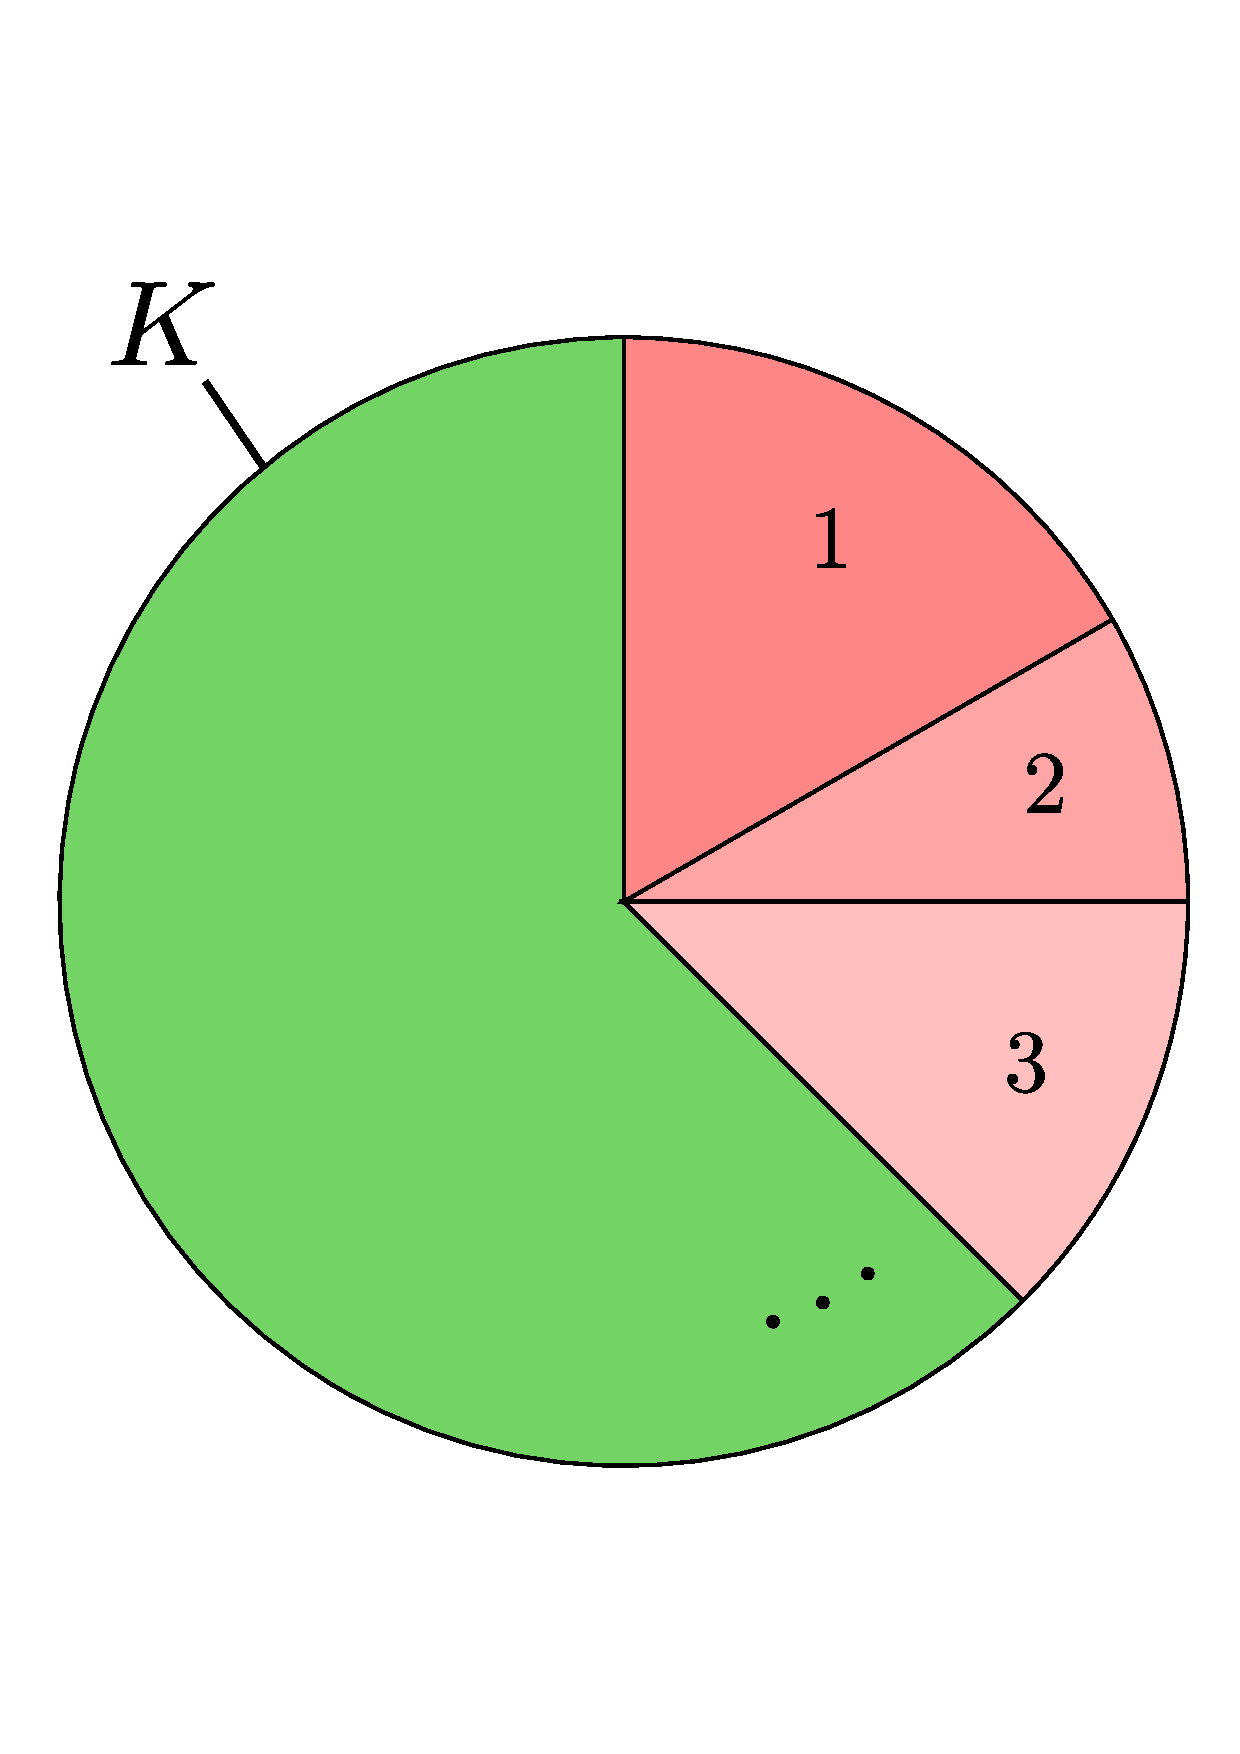
\includegraphics[height=\textheight]{semantics/img/weak_bisimulation.pdf}
	\end{center}
\end{frame}

\begin{frame}
	\frametitle{Bisimulations}
	\uncover<+->{
		\begin{definition}[Weak Bisimulation]
			Let $R$ be a binary relation.
			If $\pair{K, G} \in R$, then
			\begin{enumerate}[i)]
				\itemspacing{7pt}
				\item[] Let $G' = \wh(G)$
				\item $\resN{G'} \sqsubseteq K$
				\item $\pair{K - \resN{G'}, G'} \in R$
			\end{enumerate}
		\end{definition}
	}
	\uncover<+->{
		\begin{theorem}
			Let $R$ be a weak bisimulation.
			Then \[ \pair{K, G} \in R \land G \models B
			\implies \smtx{\while{B}{P}}(G) \sqsubseteq K \]
		\end{theorem}
	}
\end{frame}

\begin{frame}
	\frametitle{Bisimulations}
	\begin{center}
		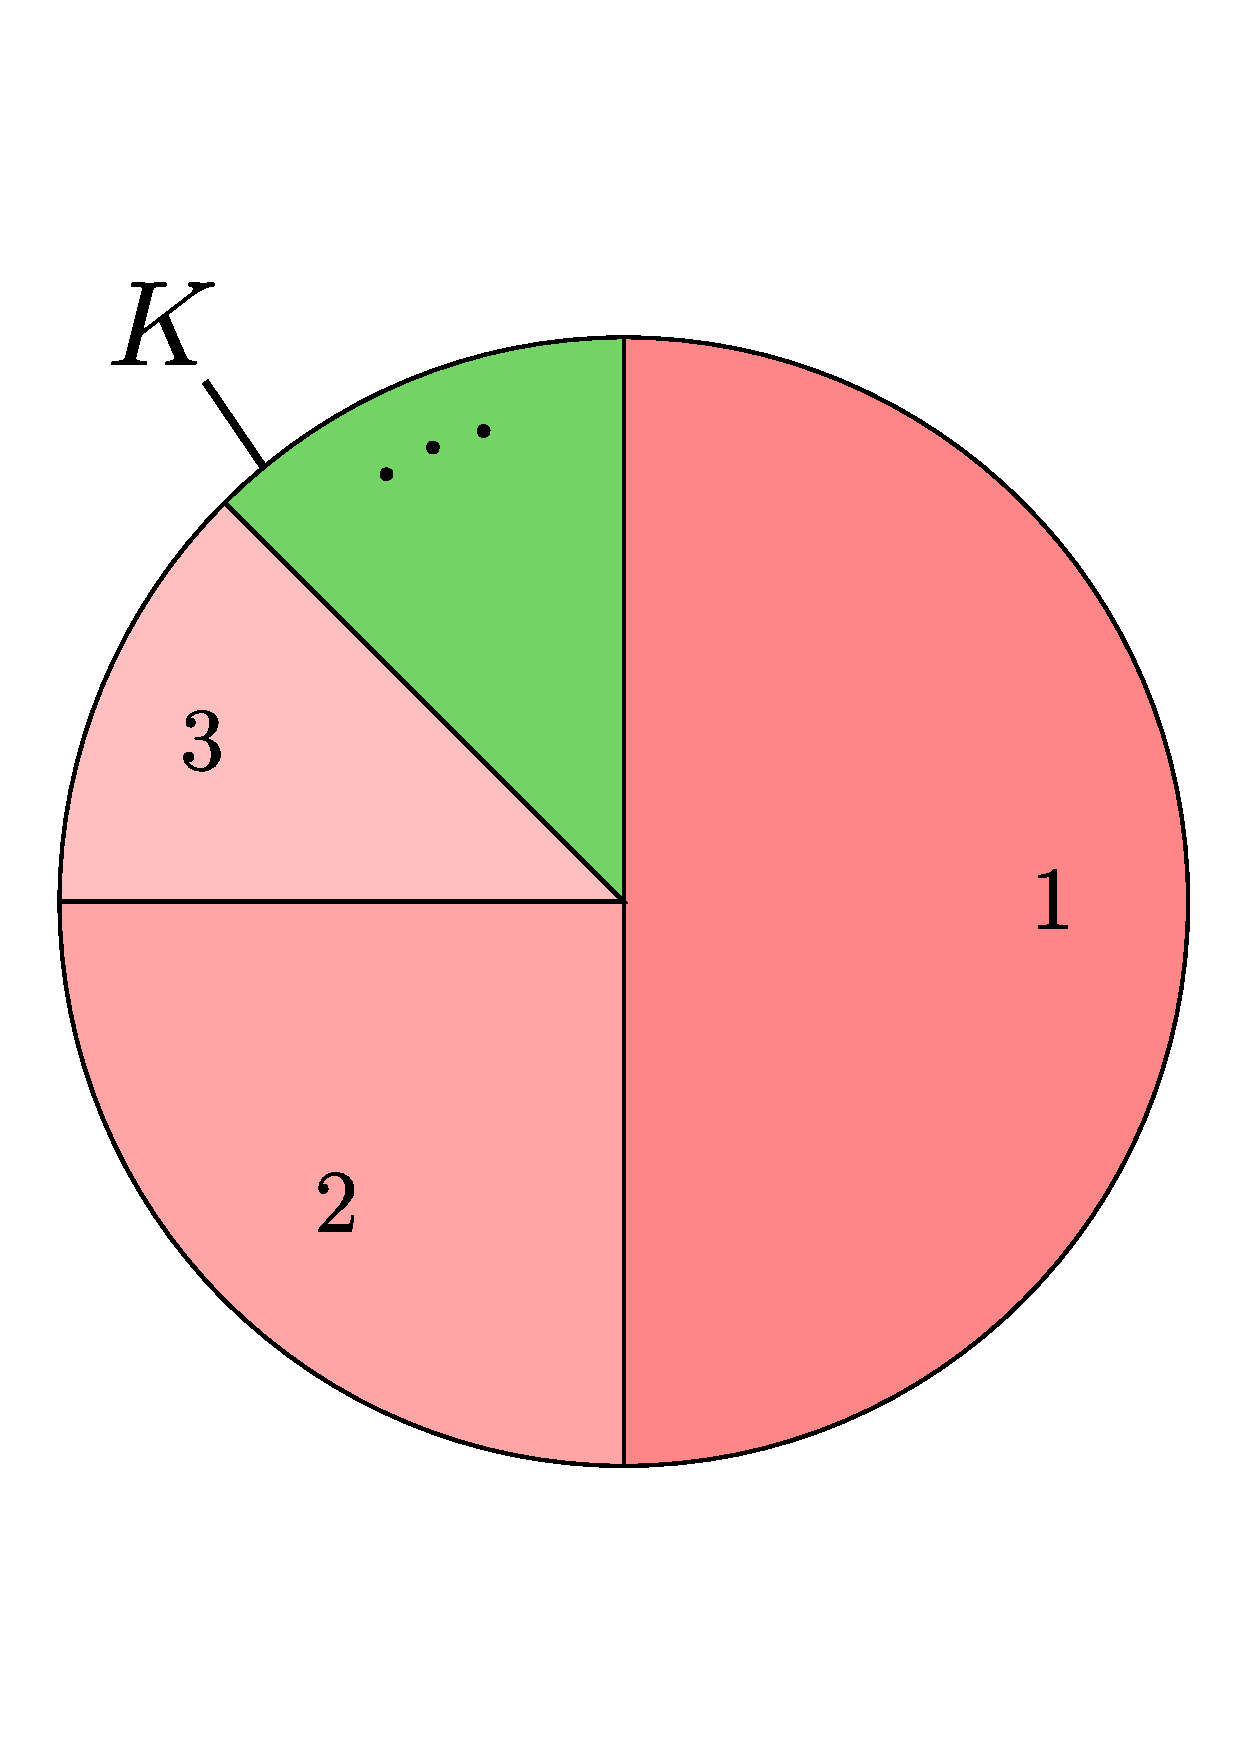
\includegraphics[height=\textheight]{semantics/img/strong_bisimulation.pdf}
	\end{center}
\end{frame}

\begin{frame}
	\frametitle{Bisimulations}
	\uncover<+->{
		\begin{definition}[Strong Bisimulation]
			Let $R$ be a binary relation and $\varepsilon \in (0, 1)$.
			If $\pair{K, G} \in R$, then
			\begin{enumerate}[i)]
				\itemspacing{7pt}
				\item[] Let $G' = \wh(G)$
				\item $\resN{G'} \leqD K$
				\item $\pair{K - \resN{G'}, G'} \in R$
				\item $\left| \resN{G'}\right| \geq \varepsilon \cdot \l| K \r|$
			\end{enumerate}
		\end{definition}
	}
	\uncover<+->{
		\begin{theorem}
			Let $R$ be a strong bisimulation.
			Then \[ \pair{K, G} \in R \land G \models B
				\implies \smtx{\while{B}{P}}(G) = K \]
		\end{theorem}
	}
\end{frame}

\begin{frame}[fragile]
	\frametitle{Bisimulations}
	\begin{lstlisting}
 while (F = 0) {
   {X := X + 1}[0.5]{F := 1}
 }
	\end{lstlisting}
	\begin{itemize}[<+->]
		\itemspacing{10pt}
		\item $ G = 1$, $ K = \frac{1}{2 - X} $
		\item Bisimulation: $ R = \l\{ \pair{K, G}  \r\} \cup
			\only<+->{
				\l\{ \pair{
					\alert<+>{ \res{\frac{1}{2 - X}}{X \geq n} },
					\alert<+>{ \half^n \cdot \l( X^n F^0 + X^{n-1} F^1 \r) } } \ 
					\middle| \ n \in \N_{>0} \r\} 
			} $
		\item $R$ is in fact a strong bisimulation ($\varepsilon = \hf$)!
		\item $ \smtx{\while{F = 0}{\ldots}}(1) \sqsubseteq K $
		\item $ \smtx{\while{F = 0}{\ldots}}(1) = K $
	\end{itemize}
\end{frame}

\newpage


\bibliographystyle{alpha}
\bibliography{literature}

\end{document}
